% \subsection{\texorpdfstring{\Zone}{Z1} Mass Constraint}  % TODO: Makes Z1 in subsection title NOT bold.
\subsection{Refitting muon and electron \pt with a \texorpdfstring{\Zone}{Z1} Mass Constraint}  % TODO: Makes Z1 in subsection title NOT bold.
% % \subsection{\texorpdfstring{\boldmath{\Zone}}{Z1} Mass Constraint} % TODO: Although \boldmath makes \subsection bold, it also makes the TOC entry bold.
\label{sec:Z1constraint}

%\subsubsection{Z1-mass line shape}
% \subsubsection{Methodology}
% TODO:REWORD, USE CONSISTENT SYMBOLS.
In order to improve the four lepton invariant mass resolution, a kinematic fit is also performed
using a mass constraint on the intermediate on-shell Z resonance, using an approach similar to the one
described previously.
% TODO:CITE
% \cite{RefToZrefit}.
The basic idea is to re-evaluate \pT of two leptons forming 
the Z bosons of the Higgs candidate, with a constraint on the reconstructed Z mass to follow 
the Z boson true lineshape. For a 125 \GeV Higgs, the selected $Z_{1}$ is mostly on-shell, 
while $m_{Z_{2}}$ distribution is broad and the spread is much bigger than detector resolution. 
When considering mass measurment of 125 \GeV Higgs, expected gain in resolution comes from refitting $Z_{1}$.
The likelihood to be maximized can be written as:
\[
\mathcal{L}(p_{T}^{1} , p_{T}^{2}|p_{T}^{reco1}, \sigma p_{T}^{1},p_{T}^{reco2}, \sigma p_{T}^{2}) = 
Gauss(p_{T}^{reco1}|p_{T}^{1}, \sigma p_{T}^{1}) \cdot Gauss(p_{T}^{reco2}|p_{T}^{2}, \sigma p_{T}^{2}) 
\cdot \mathcal{L}(m_{12}|m_{Z},m_{H})
\]
where $p_{T}^{reco1,2}$ are the reconstructed transverse momentum of the two leptons forming the $Z_{1}$,
$\sigma_{p_{T}^{1,2}}$ are the per lepton resolution (uncertainty on \pT measurement, corrected using 
method described in \ref{sec:ebe}), $p_{T}^{1,2}$ are the observables under optimisation,
$m_{12}$ is the invariant mass calculated from $p_{T}^{1}$ and $p_{T}^{2}$. $\mathcal{L}(m_{12}|m_{Z},m_{H})$
is the likelihood, given the true lineshape of $m_{Z_{1}}$. \\
%For a 125 \GeV Higgs, the selected $Z_{1}$ is not always on-shell, so the Breit Wigner shape can not describe
%perfectly its lineshape at generator level. In principle, one can choose any of the $Z_{1}$ 
%lineshapes to be used in the refitting procedure. As long as all Monte Carlor samples and data
%events go through the same procedure (including the same true $Z_{1}$ lineshape), 
%no bias would be introduced.  We choose true gen level $Z_{1}$ lineshape from the SM Higgs boson sample to
%optimize the sensitivity.
For each event, the likelihood is maximized and \pT information of the refitted leptons are updated. \\
Fig.~\ref{fig:Z1_lineshape} shows the on-shell Z resonance line shape, at generator level, 
used to perform the kinematical fit, as taken from ggH 125 \GeV sample. 
Events from all three years have been merged, asking for a 
$p_T > 20(10)$\GeV for (sub)leading leptons, and $|\eta|<$2.4(2.5) for $\mu$(e), focusing on
the reconstructed mass range of [105-140] \GeV in $m_{4l}^{RECO}$. The fit function used is a convolution
of a CB plus three different guassians.
\begin{multiFigure}[!htbp]
    \centering
	\addFigure{0.45}{../../higgsmassmeasurement/AN-19-248/Figures/Z1_lineshape/4mu.pdf}
	\addFigure{0.45}{../../higgsmassmeasurement/AN-19-248/Figures/Z1_lineshape/4e.pdf}
  	\addFigure{0.45}{../../higgsmassmeasurement/AN-19-248/Figures/Z1_lineshape/2e2mu.pdf}
	\addFigure{0.45}{../../higgsmassmeasurement/AN-19-248/Figures/Z1_lineshape/2mu2e.pdf}
	\captionof{figure}
        [On-shell Z resonance line shape at generator level, as taken from ggH sample @ 125 \GeV]
        {On-shell Z resonance line shape at generator level, as taken from ggH sample @ 125 \GeV, % TODO:REWORD
        merging all three years for the 4 different final states:
        \;A) 4$\mu$.
        \;B) 4e.
        \;C) 2e2$\mu$.
        \;D) 2$\mu$2e.
        }
    \label{fig:Z1_lineshape}
\end{multiFigure}
%After this kinimatic refitting, the mass of the Z candidate, the $m_{4\ell}$, and the $\sigma_{m_{4\ell}}$
%are recalculated. The comparison of the reconstructed and refitted mass can be seen in Fig.~\ref{Z1constraint}.
%\begin{figure}[!htbp]
%	\begin{center}
%		\subfloat[][2016]
%		   {		\includegraphics[width=0.35\textwidth]{../../higgsmassmeasurement/AN-19-248/Figures/Placeholder.png}
%					\includegraphics[width=0.35\textwidth]{../../higgsmassmeasurement/AN-19-248/Figures/Placeholder.png} 
%					\includegraphics[width=0.35\textwidth]{../../higgsmassmeasurement/AN-19-248/Figures/Placeholder.png}
%			}\\
%		\subfloat[][2017]
%		   {		\includegraphics[width=0.35\textwidth]{../../higgsmassmeasurement/AN-19-248/Figures/Placeholder.png}
%					\includegraphics[width=0.35\textwidth]{../../higgsmassmeasurement/AN-19-248/Figures/Placeholder.png} 
%					\includegraphics[width=0.35\textwidth]{../../higgsmassmeasurement/AN-19-248/Figures/Placeholder.png}
%			}\\
%		\subfloat[][2018]
%		   {		\includegraphics[width=0.35\textwidth]{../../higgsmassmeasurement/AN-19-248/Figures/Placeholder.png}
%					\includegraphics[width=0.35\textwidth]{../../higgsmassmeasurement/AN-19-248/Figures/Placeholder.png} 
%					\includegraphics[width=0.35\textwidth]{../../higgsmassmeasurement/AN-19-248/Figures/Placeholder.png}
%			}
%		\caption{Comparison of reconstructed and refitting four-lepton mass for different final states
%		of $m_{H}$ = 125GeV MC sample. 4$\mu$ on the left, 4e in the middle and 2e2$\mu$ on the right.}
%	\label{Z1constraint}
%	\end{center}
%\end{figure}
%%%%%%%%%%%%%%%%
%%%%%%%%%%%%%%%%
%%%%%%%%%%%%%%%%
%%%%%%%%%%%%%%%%
%%% move these plots after EBE %%%
%%%%%%%%%%%%%%%%
%%%%%%%%%%%%%%%%
%%%%%%%%%%%%%%%%
%%%%%%%%%%%%%%%%
%A comparison between measured $\sigma_{m_{4\ell}}$ and prediction after refitting, following 
%same procedure as described in \ref{sec:ClosureTest}, is performed. 
%Fig.~\ref{closure_Z1constraint} shows the closure test after refitting procedure.
%\begin{figure}[!htbp]
%	\begin{center}
%		\subfloat[][2016]
%		   {		\includegraphics[width=0.35\textwidth]{../../higgsmassmeasurement/AN-19-248/Figures/Z1Refit/2016_Z1Refit_H4mu_Closure_test.png}
%					\includegraphics[width=0.35\textwidth]{../../higgsmassmeasurement/AN-19-248/Figures/Z1Refit/2016_Z1Refit_H4e_Closure_test.png} 
%					\includegraphics[width=0.35\textwidth]{../../higgsmassmeasurement/AN-19-248/Figures/Z1Refit/2016_Z1Refit_H2e2mu_Closure_test.png}
%			}\\
%		\subfloat[][2017]
%		   {		\includegraphics[width=0.35\textwidth]{../../higgsmassmeasurement/AN-19-248/Figures/Z1Refit/2017_Z1Refit_H4mu_Closure_test.png}
%					\includegraphics[width=0.35\textwidth]{../../higgsmassmeasurement/AN-19-248/Figures/Z1Refit/2017_Z1Refit_H4e_Closure_test.png} 
%					\includegraphics[width=0.35\textwidth]{../../higgsmassmeasurement/AN-19-248/Figures/Z1Refit/2017_Z1Refit_H2e2mu_Closure_test.png}
%			}\\
%		\subfloat[][2018]
%		   {		\includegraphics[width=0.35\textwidth]{../../higgsmassmeasurement/AN-19-248/Figures/Z1Refit/2018_Z1Refit_H4mu_Closure_test.png}
%					\includegraphics[width=0.35\textwidth]{../../higgsmassmeasurement/AN-19-248/Figures/Z1Refit/2018_Z1Refit_H4e_Closure_test.png} 
%					\includegraphics[width=0.35\textwidth]{../../higgsmassmeasurement/AN-19-248/Figures/Z1Refit/2018_Z1Refit_H2e2mu_Closure_test.png}
%			}
%		\caption{Closure test after $Z_{1}$ constraint, for different final states
%		of $m_{H}$ = 125GeV MC sample. 4$\mu$ on the left, 4e in the middle and 2e2$\mu$ on the right.}
%	\label{closure_Z1constraint}
%	\end{center}
%\end{figure}
%%%%%%%%%%%%%%%%
%%%%%%%%%%%%%%%%
%%%%%%%%%%%%%%%%
%%%%%%%%%%%%%%%%



%\subsubsection{Refitted pT with constraints} 
%The constraint of the Z boson has been also implemented using new muon reconstruction (VX+BS),
%following the procedure described in the previous paragraph.
%Fig.~\ref{Mass_comparison_4mu} shows H boson mass distribution (105-140 GeV) using  
%four different approaches: baseline, Refitted\_baseline (aka baseline and Z boson constraint),
%VX+BS and Refitted\_VXBS (aka VX+BS and Z boson constraint). As can be seen, 
%all different production
%modes benefits from the inclusion of the VX+BS constraint living the yields unchanged. 
%The VX+BS helps not only 4$\mu$ final state but also 2e2$\mu$ and 2$\mu$2e as can be seen in 
%~Fig.~\ref{Mass_comparison_2e2mu}. The 4e final state is instead not affected 
%~Fig.~\ref{Mass_comparison_4e} since electron information are not updated after VX+BS.
%\begin{figure}[!htbp]
%\begin{center}
%	\includegraphics[width=0.35\textwidth]{../../higgsmassmeasurement/AN-19-248/Figures/Placeholder.png}
%	\includegraphics[width=0.35\textwidth]{../../higgsmassmeasurement/AN-19-248/Figures/Placeholder.png} 
%	\includegraphics[width=0.35\textwidth]{../../higgsmassmeasurement/AN-19-248/Figures/Placeholder.png} 
%	\includegraphics[width=0.35\textwidth]{../../higgsmassmeasurement/AN-19-248/Figures/Placeholder.png}
%	\includegraphics[width=0.35\textwidth]{../../higgsmassmeasurement/AN-19-248/Figures/Placeholder.png} 
%	\includegraphics[width=0.35\textwidth]{../../higgsmassmeasurement/AN-19-248/Figures/Placeholder.png} 
%\caption{H boson mass distribution for 2016 on top (ggH on the left WH on the right),
%2017 in the middle (ggH on the left ZH on the right),
%2018 on bottom (ggH on the left VBF on the right).
%Four different approaches are shown: baseline (black), refit+baseline (red), VXBS (green)
%and VXBS+refit (blue).}
%\label{Mass_comparison_4mu}
%\end{center}
%\end{figure}
%\begin{figure}[!htbp]
%\begin{center}
%	\includegraphics[width=0.35\textwidth]{../../higgsmassmeasurement/AN-19-248/Figures/Placeholder.png}
%	\includegraphics[width=0.35\textwidth]{../../higgsmassmeasurement/AN-19-248/Figures/Placeholder.png} 
%	\includegraphics[width=0.35\textwidth]{../../higgsmassmeasurement/AN-19-248/Figures/Placeholder.png} 
%	\includegraphics[width=0.35\textwidth]{../../higgsmassmeasurement/AN-19-248/Figures/Placeholder.png}
%	\includegraphics[width=0.35\textwidth]{../../higgsmassmeasurement/AN-19-248/Figures/Placeholder.png} 
%	\includegraphics[width=0.35\textwidth]{../../higgsmassmeasurement/AN-19-248/Figures/Placeholder.png} 
%\caption{H boson mass distribution,for ggH in 2e2$\mu$ on the left and 2$\mu$2mu on the right, 
%for 2016 on top, 2017 in the middle, 2018 on bottom .
%Four different approaches are shown: baseline (black), refit+baseline (red), VXBS (green)
%and VXBS+refit (blue).}
%\label{Mass_comparison_2e2mu}
%\end{center}
%\end{figure}
%\begin{figure}[!htbp]
%\begin{center}
%	\includegraphics[width=0.35\textwidth]{../../higgsmassmeasurement/AN-19-248/Figures/Placeholder.png}
%	\includegraphics[width=0.35\textwidth]{../../higgsmassmeasurement/AN-19-248/Figures/Placeholder.png} 
%	\includegraphics[width=0.35\textwidth]{../../higgsmassmeasurement/AN-19-248/Figures/Placeholder.png} 
%\caption{H boson mass distribution,for ggH in 4e final state
%for 2016 on the left, 2017 on the right, 2018 on bottom.
%Four different approaches are shown: baseline (black), refit+baseline (red), VXBS (green)
%and VXBS+refit (blue).}
%\label{Mass_comparison_4e}
%\end{center}
%\end{figure}


%=== DID NOT SHOW THESE PLOTS IN THESIS ENDORSEMENT ===%
%=== Not sure if I can show them.
% \subsubsection{Validation}
% Fig.~\ref{Z1_Higgs_Validation} shows a comparison of the Higgs boson mass resolution 
% (using ggH production mode @ 125 \GeV) in the three diferent approaches used so far:
% baseline (red), baseline+VXBS (green), baseline+VXBS+Z1 mass constraint (blue). There is a good 
% agreement between measured and predicted resolution which is also reduced step by
% step from baseline to full configuration (adding VXBS and Z1 constraint).
% \begin{figure}[!htbp]
% \begin{center}
% 	\includegraphics[width=0.45\textwidth]{../../higgsmassmeasurement/AN-19-248/Figures/SigmaMeas_VS_SigmaPred/4mu.pdf}
% 	\includegraphics[width=0.45\textwidth]{../../higgsmassmeasurement/AN-19-248/Figures/SigmaMeas_VS_SigmaPred/4e.pdf}
%   	\includegraphics[width=0.45\textwidth]{../../higgsmassmeasurement/AN-19-248/Figures/SigmaMeas_VS_SigmaPred/2e2mu.pdf}
% 	\includegraphics[width=0.45\textwidth]{../../higgsmassmeasurement/AN-19-248/Figures/SigmaMeas_VS_SigmaPred/2mu2e.pdf}
% \caption{Measured and predicted four-lepton invariant mass resolution using 2018 ggH sample
% 	@ 125 \GeV, in the baseline (red), baseline+VXBS (green), baseline+VXBS+Z1 mass constraint (blue)
% 	approach: 4$\mu$ (top left),
% 4e (top right), 2e2$\mu$ (bottom left), 2$\mu$2e (bottom right).}
% \label{Z1_Higgs_Validation}
% \end{center}
% \end{figure}

% \subsection{Mass distributions}
The new invariant mass distributions, with also the constraint of the on-shell Z1 boson, are shown in 
Fig.~\ref{fig:1D_VXBS_Z1_mass_2018_ggH}.
\begin{multiFigure}[!htbp]
    \centering
	\addFigure{0.45}{figures/higgsmassmeas/ggH_MassDistribution/1D_VXBS_Z1_mass_2018_ggH_4mu.pdf}
	\addFigure{0.45}{figures/higgsmassmeas/ggH_MassDistribution/1D_VXBS_Z1_mass_2018_ggH_4e.pdf}
  	\addFigure{0.45}{figures/higgsmassmeas/ggH_MassDistribution/1D_VXBS_Z1_mass_2018_ggH_2e2mu.pdf}
	\addFigure{0.45}{figures/higgsmassmeas/ggH_MassDistribution/1D_VXBS_Z1_mass_2018_ggH_2mu2e.pdf}
    \captionof{figure}
        [Four-lepton invariant mass distribution, with VXBS and Z1 constraint]
        {Four-lepton invariant mass distribution, with VXBS and Z1 constraint, in the signal region ([105-140]\GeV) using ggH events, with the DSCB fit for 2018: % TODO:REWORD
        \;A) 4$\mu$.
        \;B) 4e.
        \;C) 2e2$\mu$.
        \;D) 2$\mu$2e.
        } 
\label{fig:1D_VXBS_Z1_mass_2018_ggH}
\end{multiFigure}
Comparing these new distributions (Fig.~\ref{fig:1D_VXBS_Z1_mass_2018_ggH}) with the previous ones (Fig.~\ref{fig:1D_VXBS_mass_2018_ggH}), it can be seen that the \Zone constraint has a bigger improvement in final states with on-shell Z boson decaying in to 2e (~30$\%$ improvement on $\sigma$ for 2e2$\mu$ and 16$\%$ for 4e) while the other two final states (4$\mu$ and 2$\mu$2e) are less affected (improvement in $\sigma$ of the other of 5$\%$).

\subsubsection{Expected mH measurement uncertainties (MC) and relative improvements}
The new four-lepton mass ($m'_{4\ell}$), shown in Fig.~\ref{fig:1D_VXBS_Z1_mass_2018_ggH},
is used to rebuild the 1D likelihood function, $\mathcal{L}$($m'_{4\ell}|m_{H}$). Signal normalisation and signal parameterization are extracted following the procedure described in \ref{sec:signal_model}.
The expected \mH measurement uncertainty, is reported in Table~\ref{table:1D_model_result_Z1} (or in Table~\ref{table:1D_model_result_Z1_year}
splitted in years).
%===
\begin{table}[ht]	
\begin{center}
    \topcaption
        [Expected Higgs boson mass uncertainty measured with 1D model, with and without
        Z1 refit for different final states]
        {Expected Higgs boson mass uncertainty measured with 1D model, with and without
        Z1 refit for different final states. All mass values are given in \MeV.
        Statistical only results are considered at this stage of the analysis.
        }
    \begin{tabular}{ccccccc}
        \hline			
    Expected uncertainty	&	4$\mu$	&	4e	&	2e2$\mu$	&2$\mu$2e	& inclusive & Rel. Improvement \\
        \hline			
        1$D'_{VXBS}$ (No bkg)	&	129	&	357	&	223	&	255	&	99	&	-8\%	\\
        1$D_{VXBS}$  (No bkg)	&	137	&	394	&	275	&	266	&	108 &	-4\%	\\
    %	1$D'_{VXBS}$ (No bkg)	&	134	&	424	&	250	&	279	&	105	&	-9\%	\\
    %	1$D_{VXBS}$  (No bkg)	&	144	&	466	&	313	&	291	&	116	&	-\\	
        %\hline
    %relative improvement	&	-	&	-	&	-	&	-	&	-	\\
        \hline
\end{tabular}
\label{table:1D_model_result_Z1}
\end{center}
\end{table}
%===
\begin{table}[ht]	
\begin{center}
    \topcaption
        [Expected Higgs boson mass uncertainty measured with 1D model, with and without
        Z1 refit for different years]
        {Expected Higgs boson mass uncertainty measured with 1D model, with and without
        Z1 refit for different years. All mass values are given in \MeV.
        Statistical only results are considered at this stage of the analysis.
        }
    \begin{tabular}{ccccc}
        \hline			
    Expected uncertainty	&	2016 pre-VFP	&	2016 post-VFP	&	2017	&	2018	\\
        \hline			
        1$D'_{VXBS}$ (No bkg)	&	266	&	276	&	182	&	148	\\
        1$D_{VXBS}$	(No bkg)	&	291	&	301	&	198	&	162	\\
    %	1$D'_{VXBS}$ (No bkg)	&	206	&	194	&	157	\\
    %	1$D_{VXBS}$	(No bkg)	&	227	&	212	&	173	\\
        \hline
    \end{tabular}
    \label{table:1D_model_result_Z1_year}
\end{center}
\end{table}

%Examples of the fits for normalisation can be observed in 
%Fig.~\ref{signal_normalization_2016}, \ref{signal_normalization_2017}, \ref{signal_normalization_2018}
%\begin{figure}[!htbp]
%\begin{center}
%  		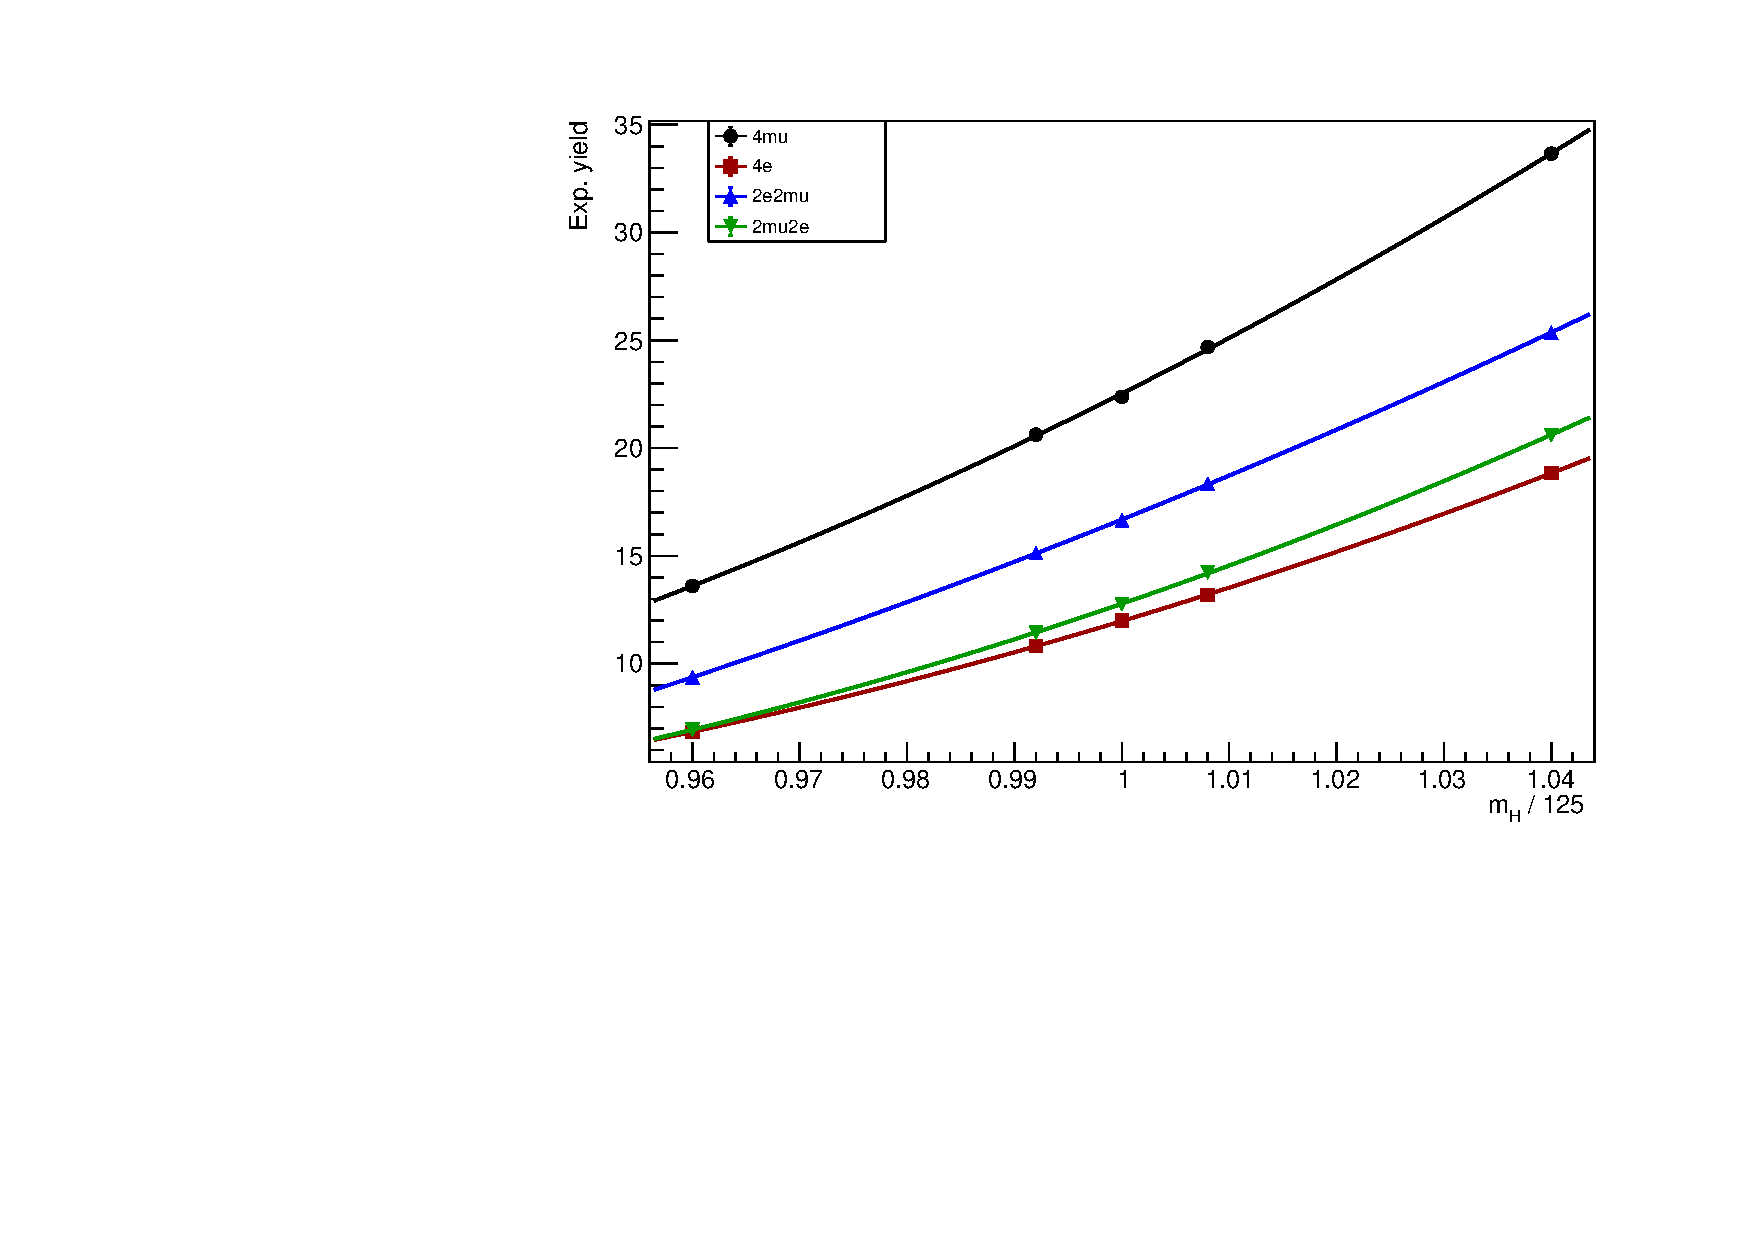
\includegraphics[width=0.3\textwidth]{../../higgsmassmeasurement/AN-19-248/Figures/SignalModelling/Signal_Normalisation/NoZ1/2016_ggH_yield.pdf}
%	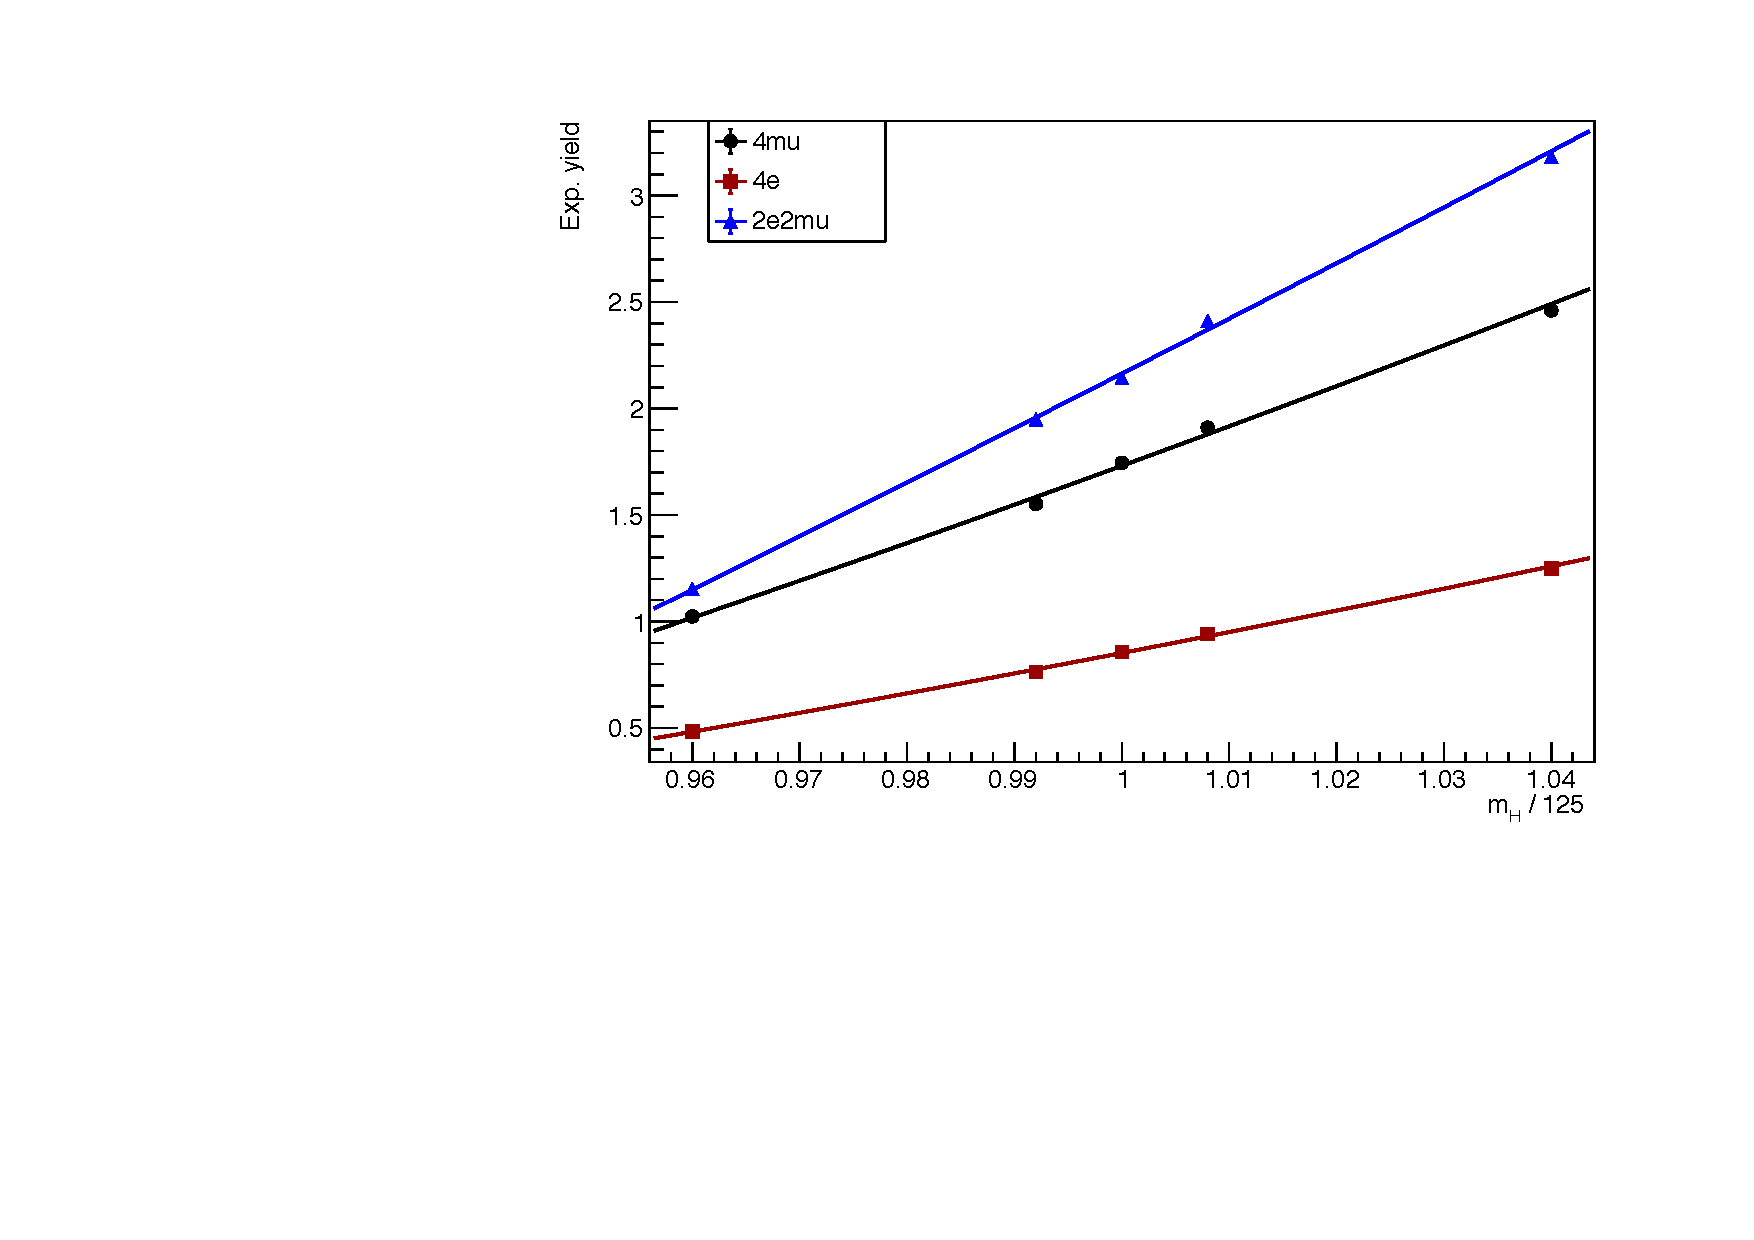
\includegraphics[width=0.3\textwidth]{../../higgsmassmeasurement/AN-19-248/Figures/SignalModelling/Signal_Normalisation/NoZ1/2016_VBF_yield.pdf} 
%	\includegraphics[width=0.3\textwidth]{../../higgsmassmeasurement/AN-19-248/Figures/SignalModelling/Signal_Normalisation/NoZ1/2016_WH_yield.pdf}
%	\caption{Normalization fit in 2016, for different decay channels, as a function
%	of mass, for ggH on the left, VBF in the middle, WH on the right.}
%\label{signal_normalization_2016}
%\end{center}
%\end{figure}
%
%\begin{figure}[!htbp]
%\begin{center}
%  		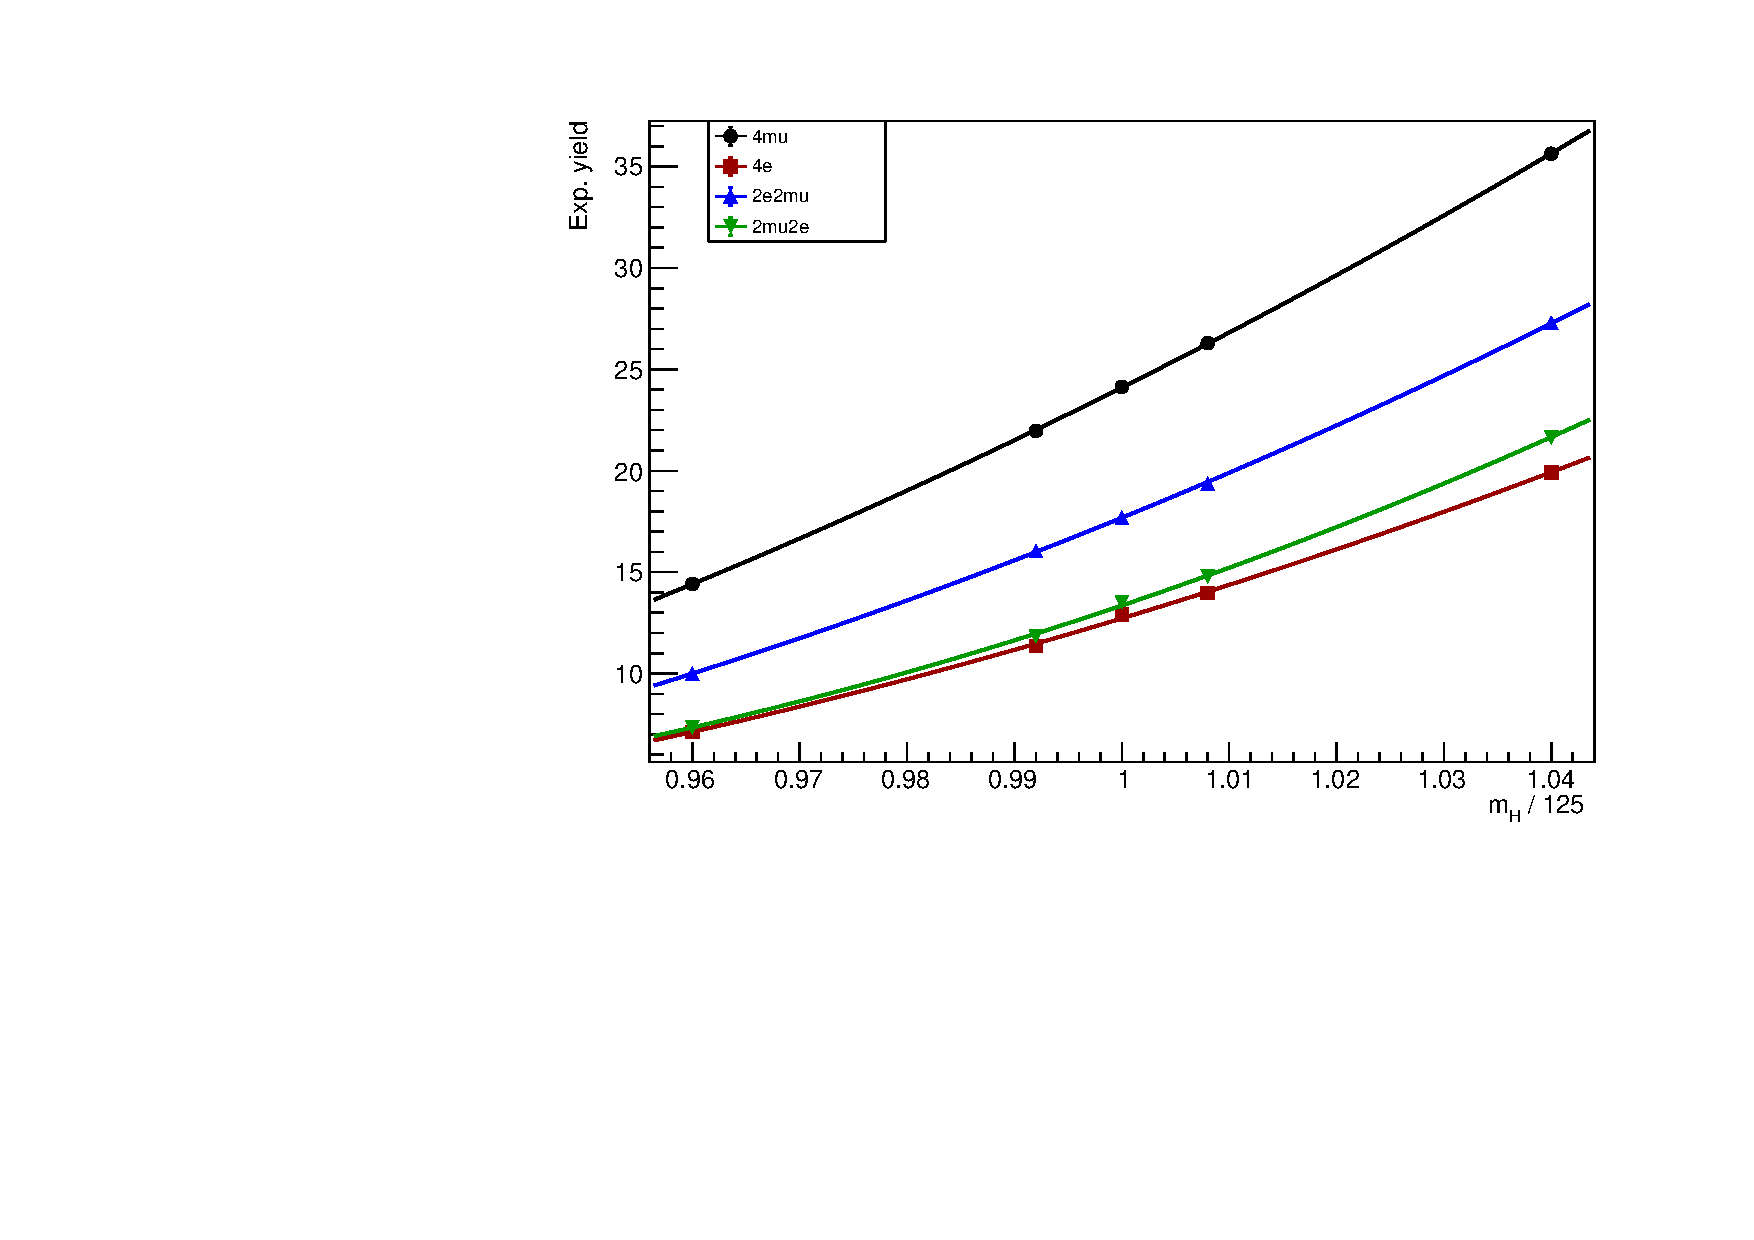
\includegraphics[width=0.3\textwidth]{../../higgsmassmeasurement/AN-19-248/Figures/SignalModelling/Signal_Normalisation/NoZ1/2017_ggH_yield.pdf}
%	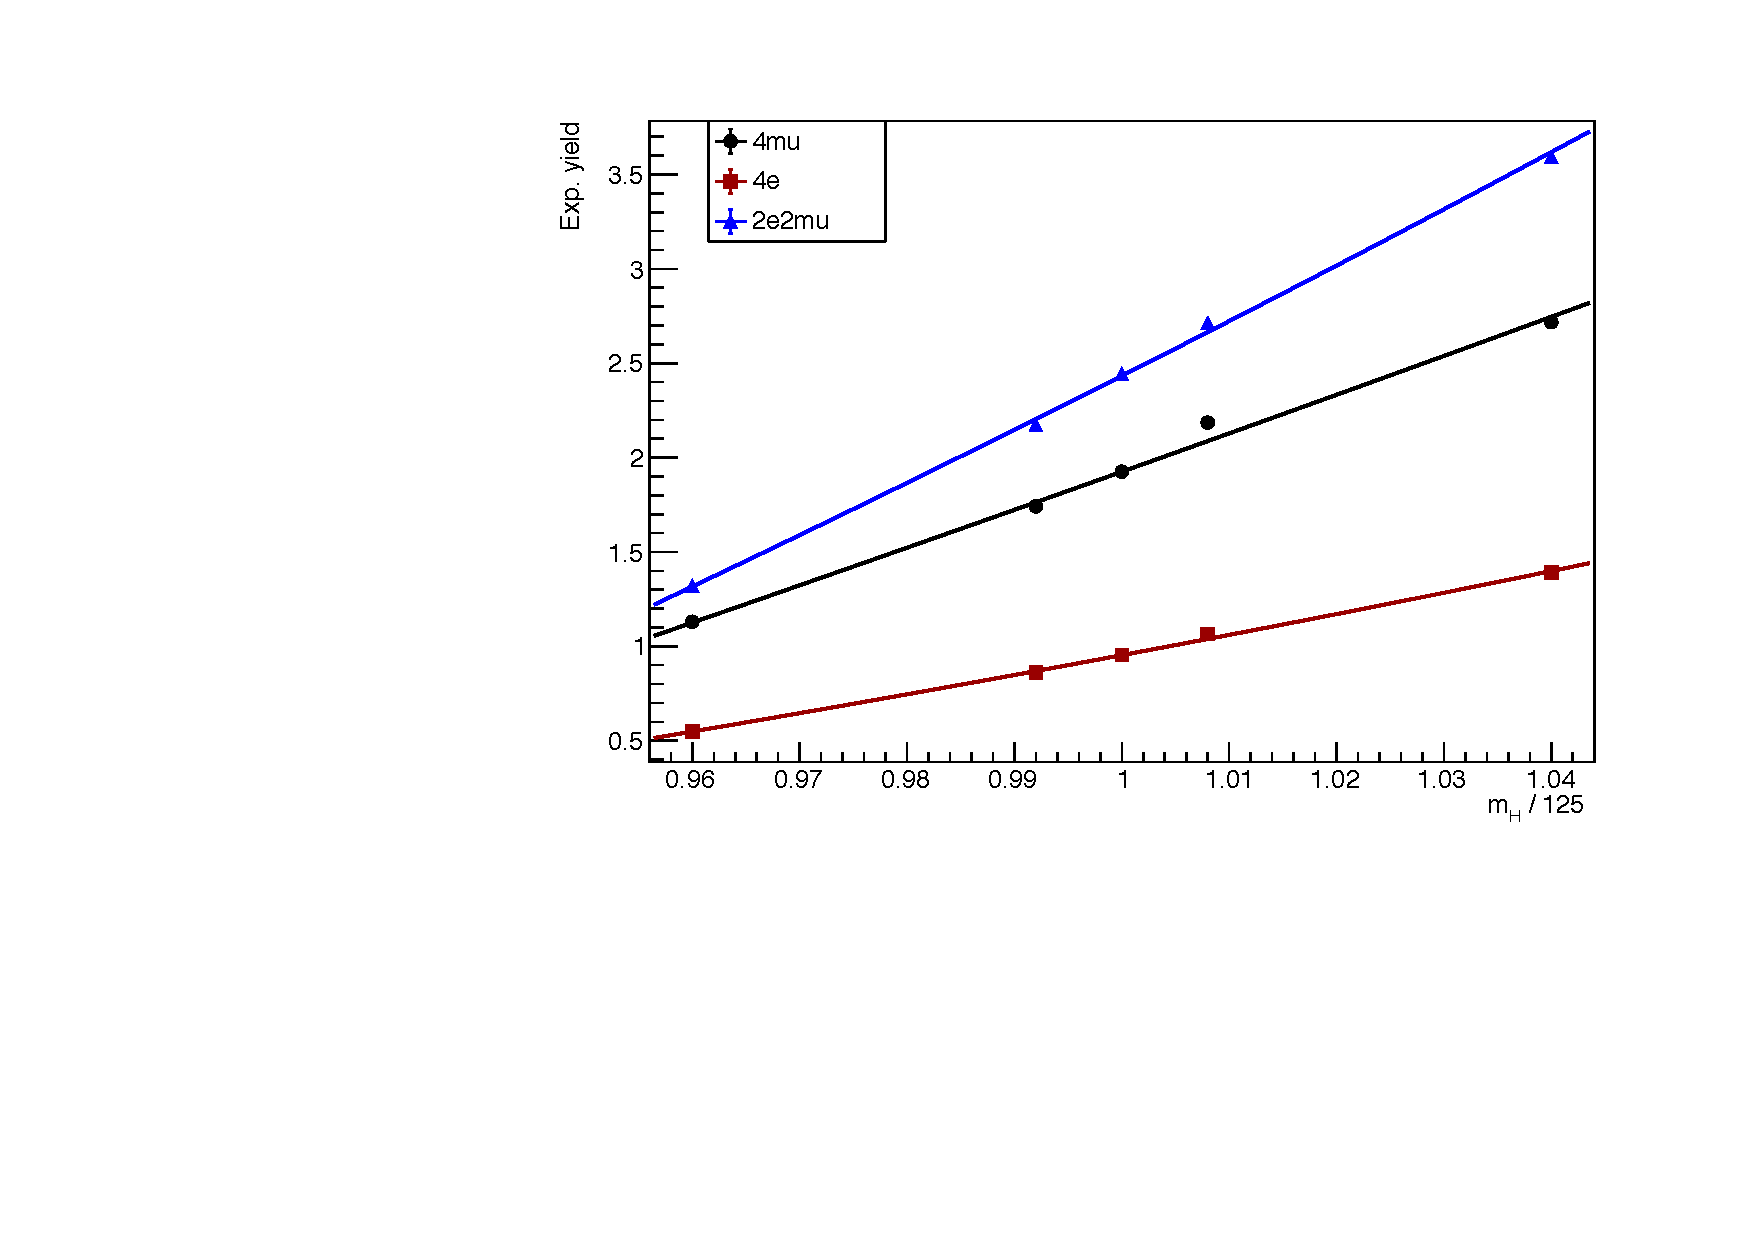
\includegraphics[width=0.3\textwidth]{../../higgsmassmeasurement/AN-19-248/Figures/SignalModelling/Signal_Normalisation/NoZ1/2017_VBF_yield.pdf} 
%	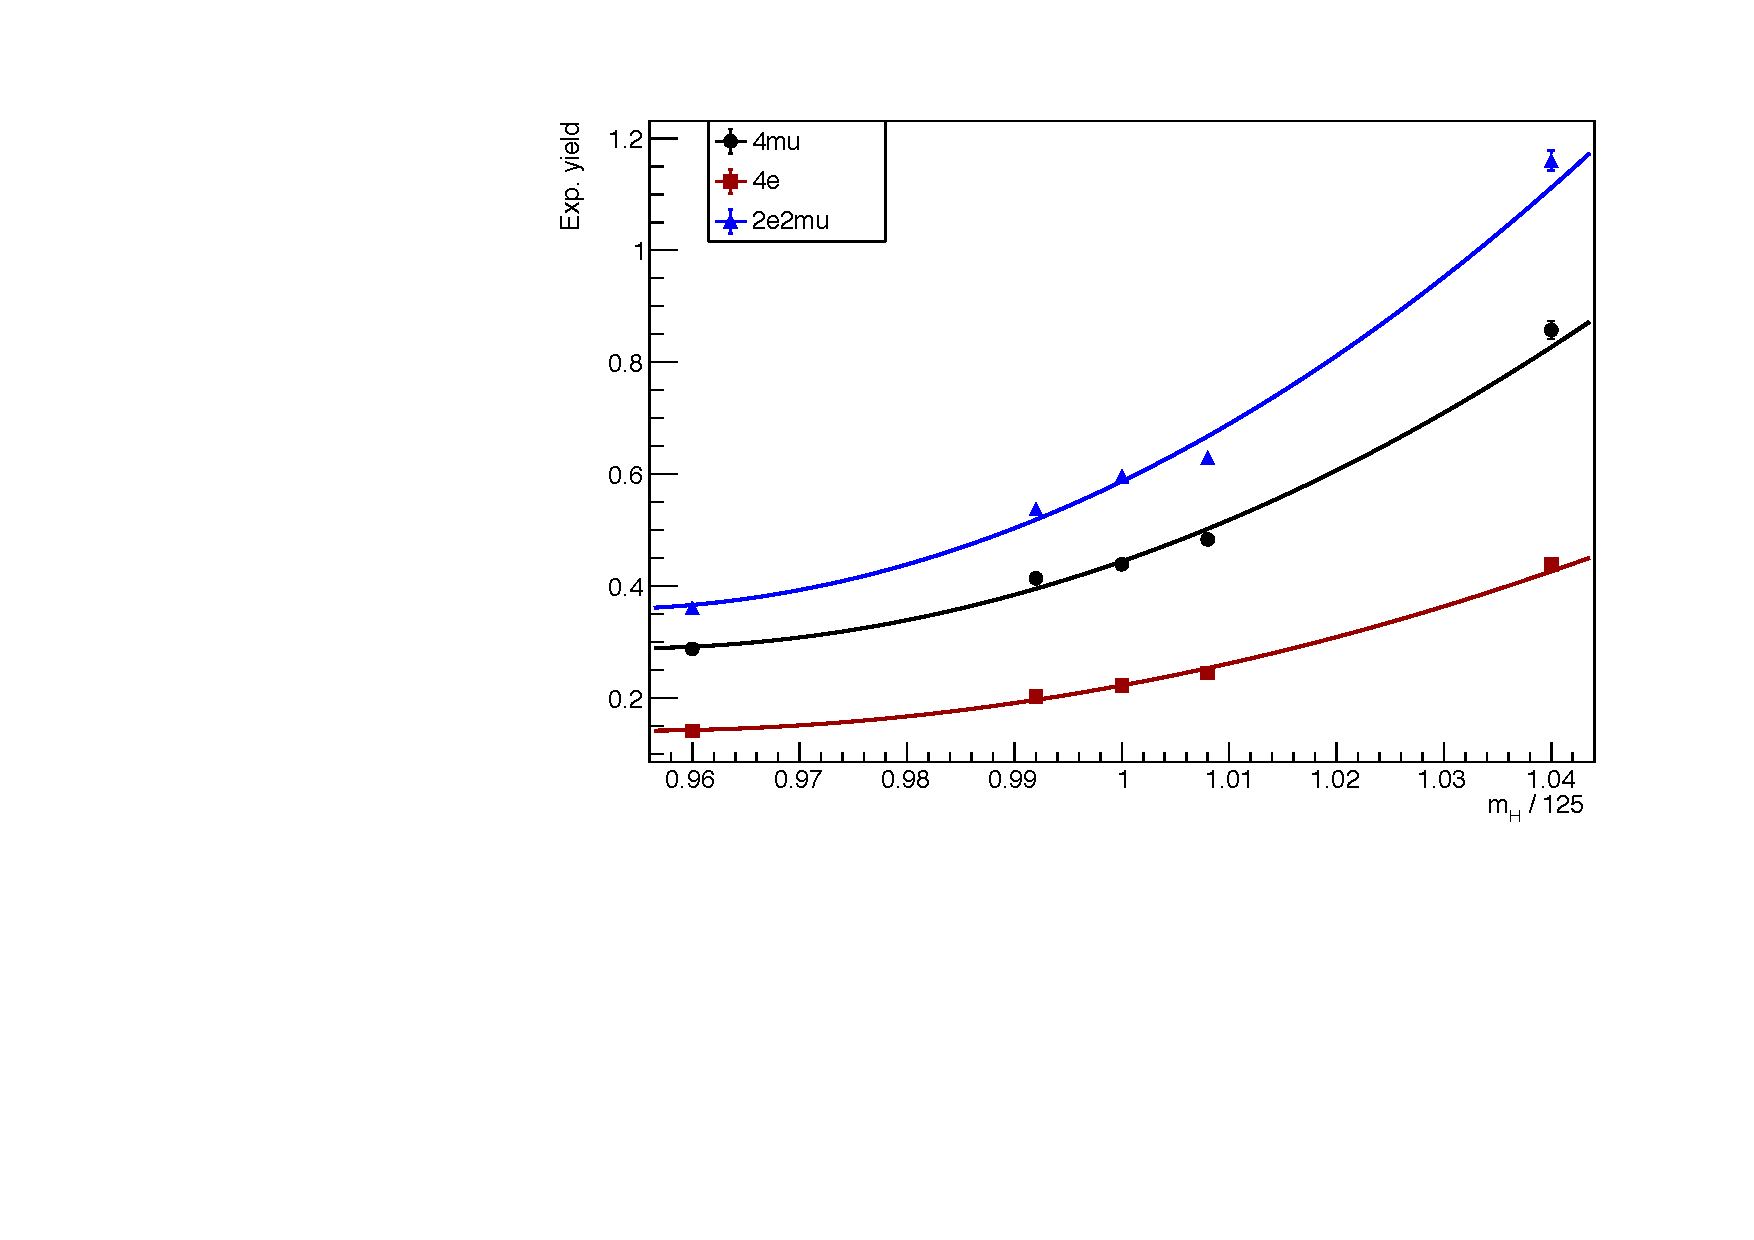
\includegraphics[width=0.3\textwidth]{../../higgsmassmeasurement/AN-19-248/Figures/SignalModelling/Signal_Normalisation/NoZ1/2017_ZH_yield.pdf}
%	\caption{Normalization fit in 2017, for different decay channels, as a function
%	of mass, for ggH on the left, VBF in the middle, ZH on the right.}
%\label{signal_normalization_2017}
%\end{center}
%\end{figure}
%
%\begin{figure}[!htbp]
%\begin{center}
%  		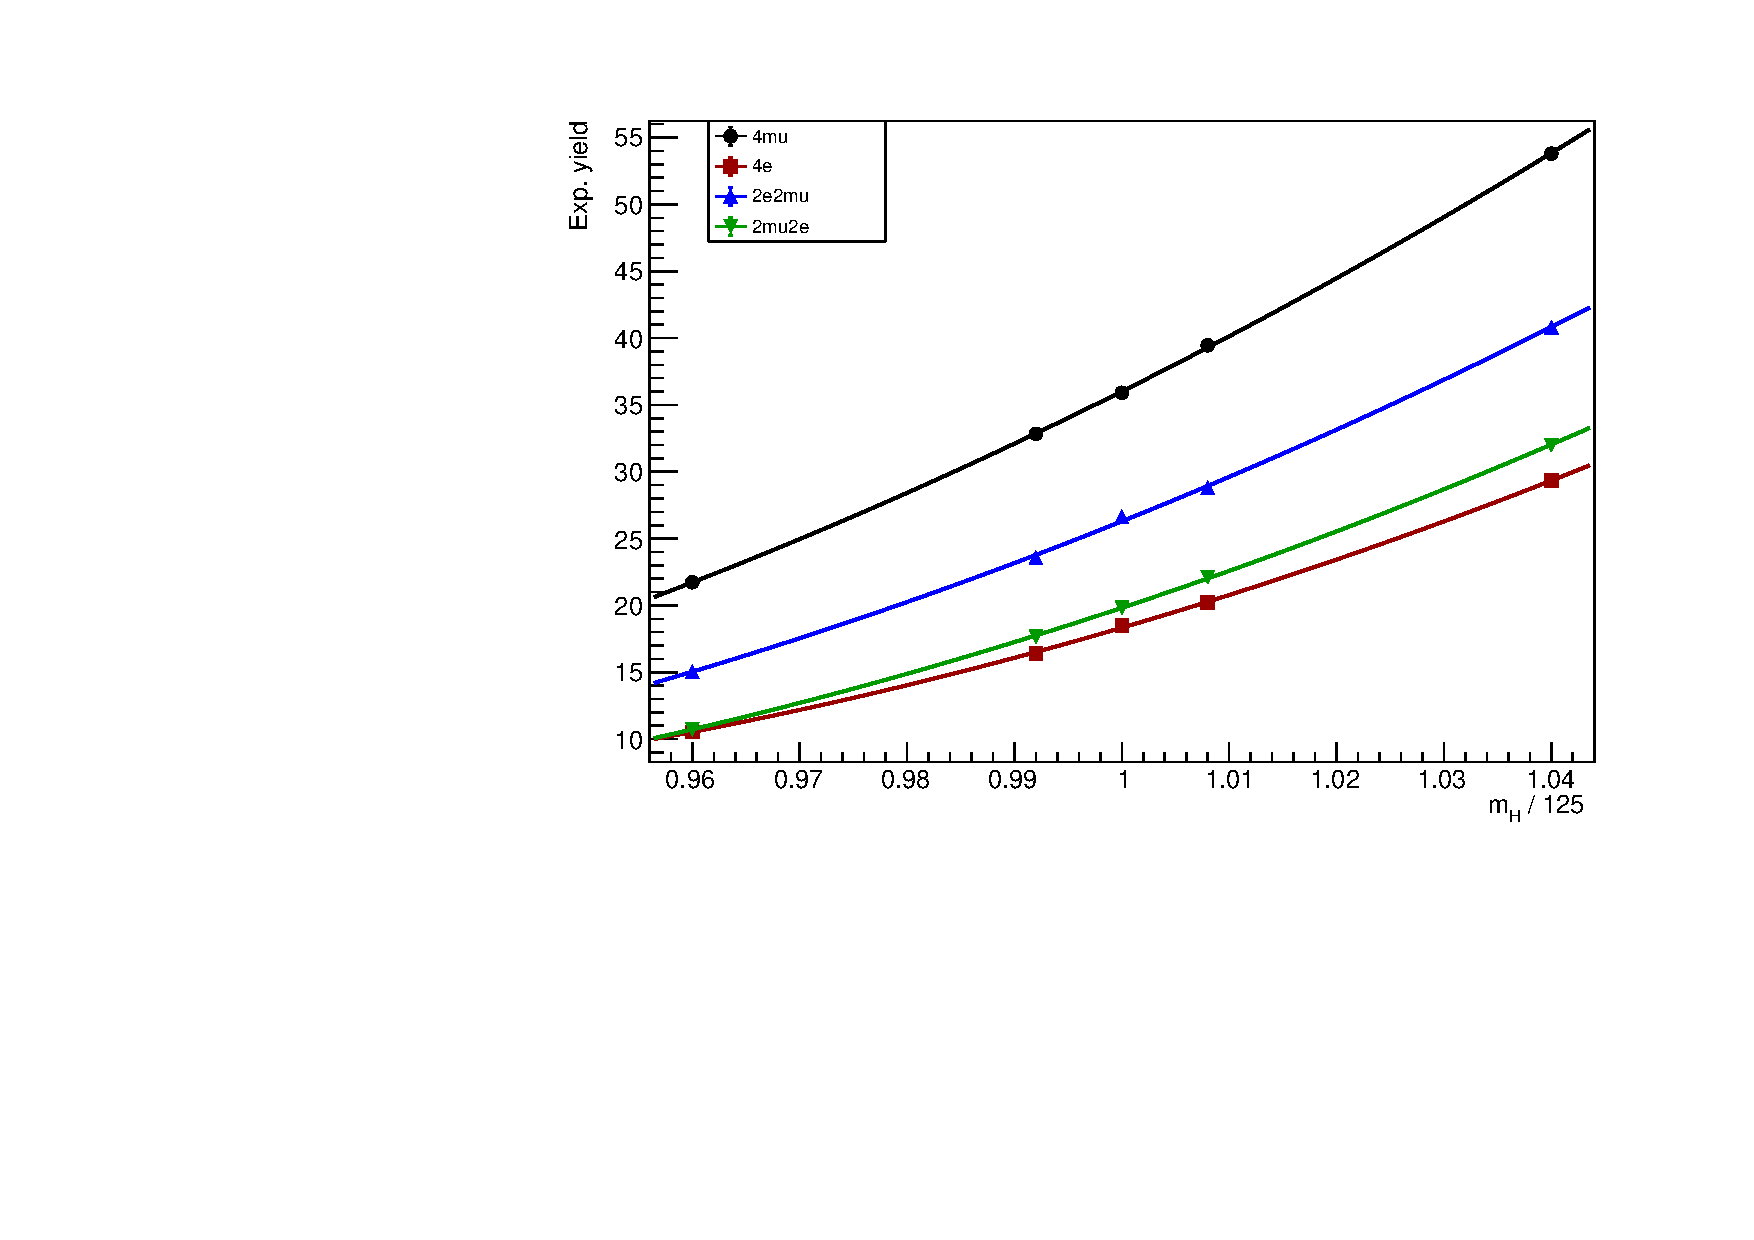
\includegraphics[width=0.3\textwidth]{../../higgsmassmeasurement/AN-19-248/Figures/SignalModelling/Signal_Normalisation/NoZ1/2018_ggH_yield.pdf}
%	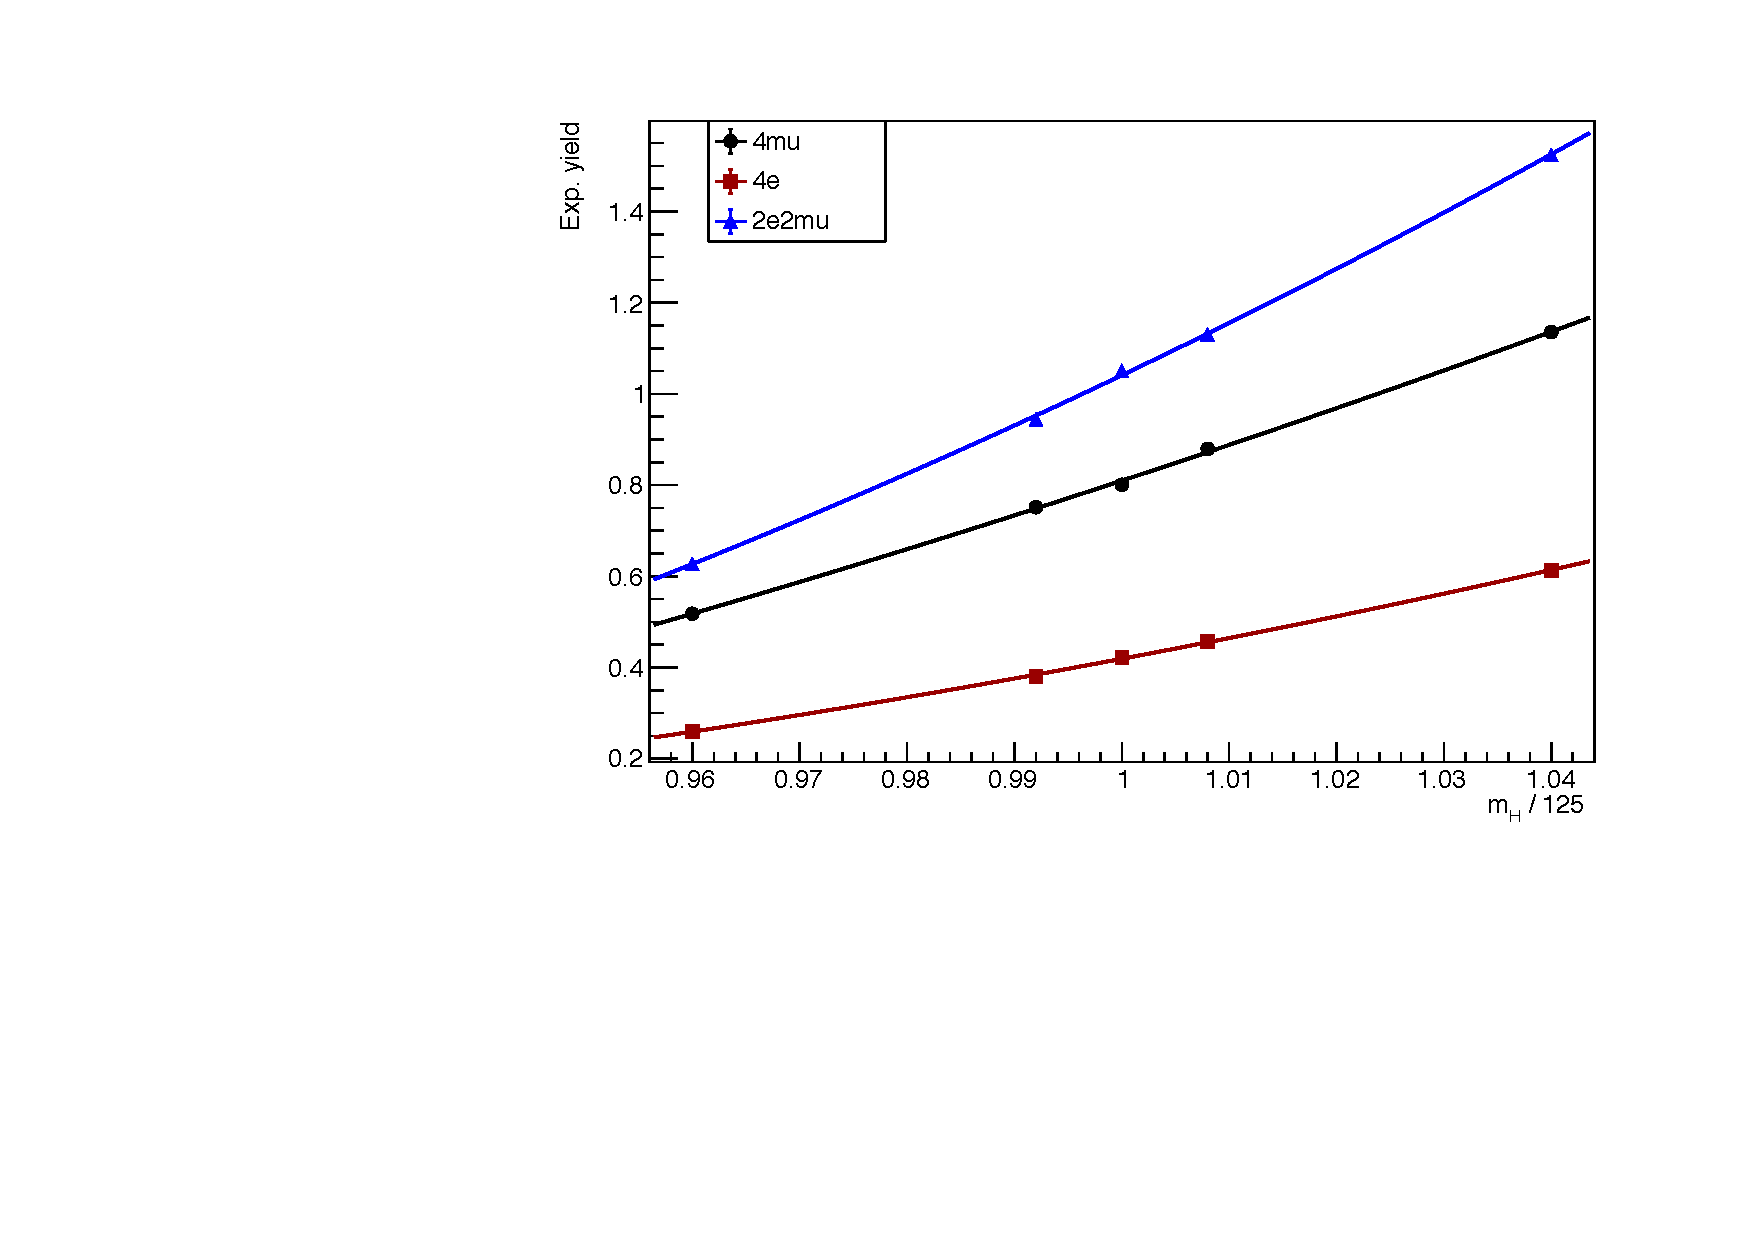
\includegraphics[width=0.3\textwidth]{../../higgsmassmeasurement/AN-19-248/Figures/SignalModelling/Signal_Normalisation/NoZ1/2018_WH_yield.pdf} 
%	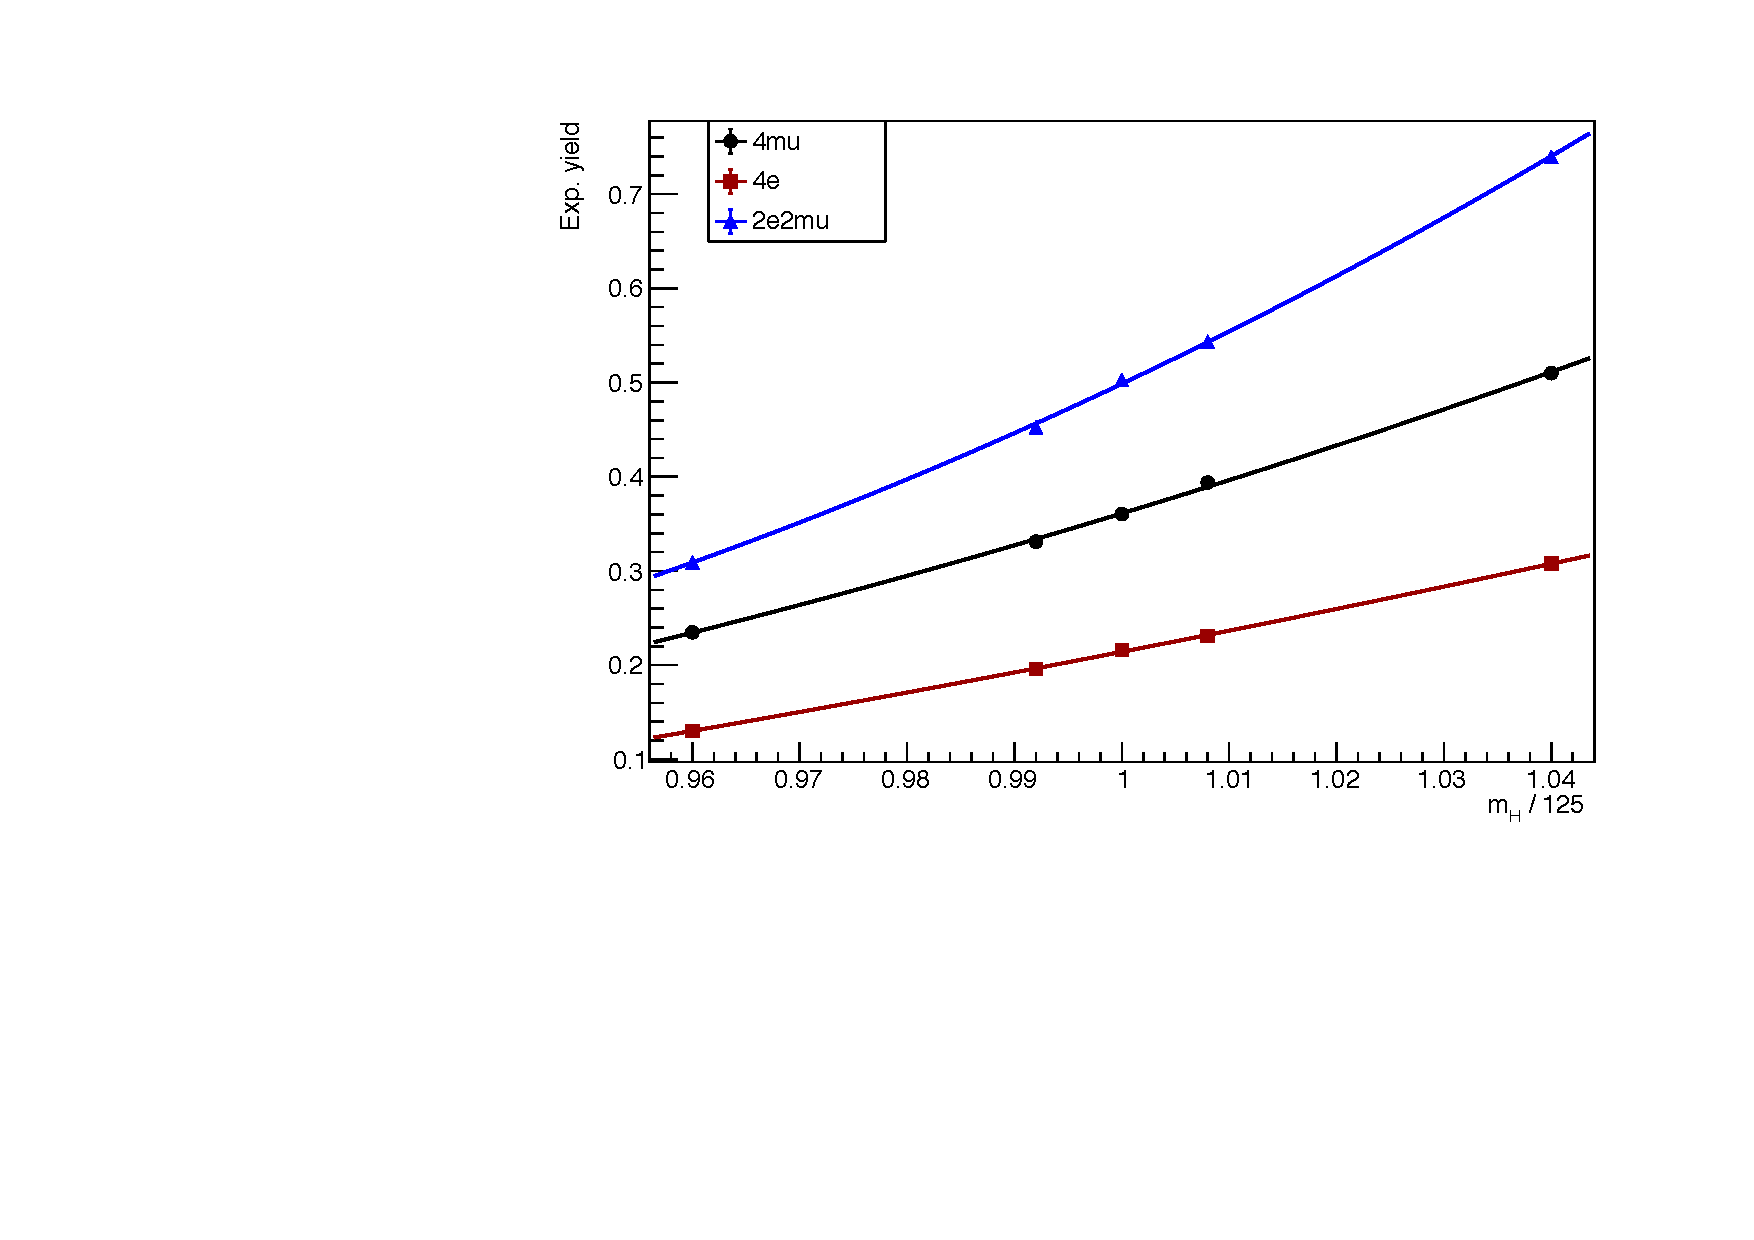
\includegraphics[width=0.3\textwidth]{../../higgsmassmeasurement/AN-19-248/Figures/SignalModelling/Signal_Normalisation/NoZ1/2018_ttH_yield.pdf}
%	\caption{Normalization fit in 2018, for different decay channels, as a function
%	of mass, for ggH on the left, WH in the middle, ttH on the right.}
%\label{signal_normalization_2018}
%\end{center}
%\end{figure}
%
%While, examples for the signal parametrisation are shown in Fig.~\ref{signal_lineshape_2016}, \ref{signal_lineshape_2017}, 
%\ref{signal_lineshape_2018} for 125 GeV sample, and in  Fig.~\ref{signal_lineshape_2016_full_1}, 
%\ref{signal_lineshape_2016_full_2}, \ref{signal_lineshape_2017_full_1}, 
%\ref{signal_lineshape_2017_full_2}, \ref{signal_lineshape_2018_full_1} and  
%\ref{signal_lineshape_2018_full_2}, for the simultaneous fits.
%\begin{figure}[!htbp]
%\begin{center}
%  		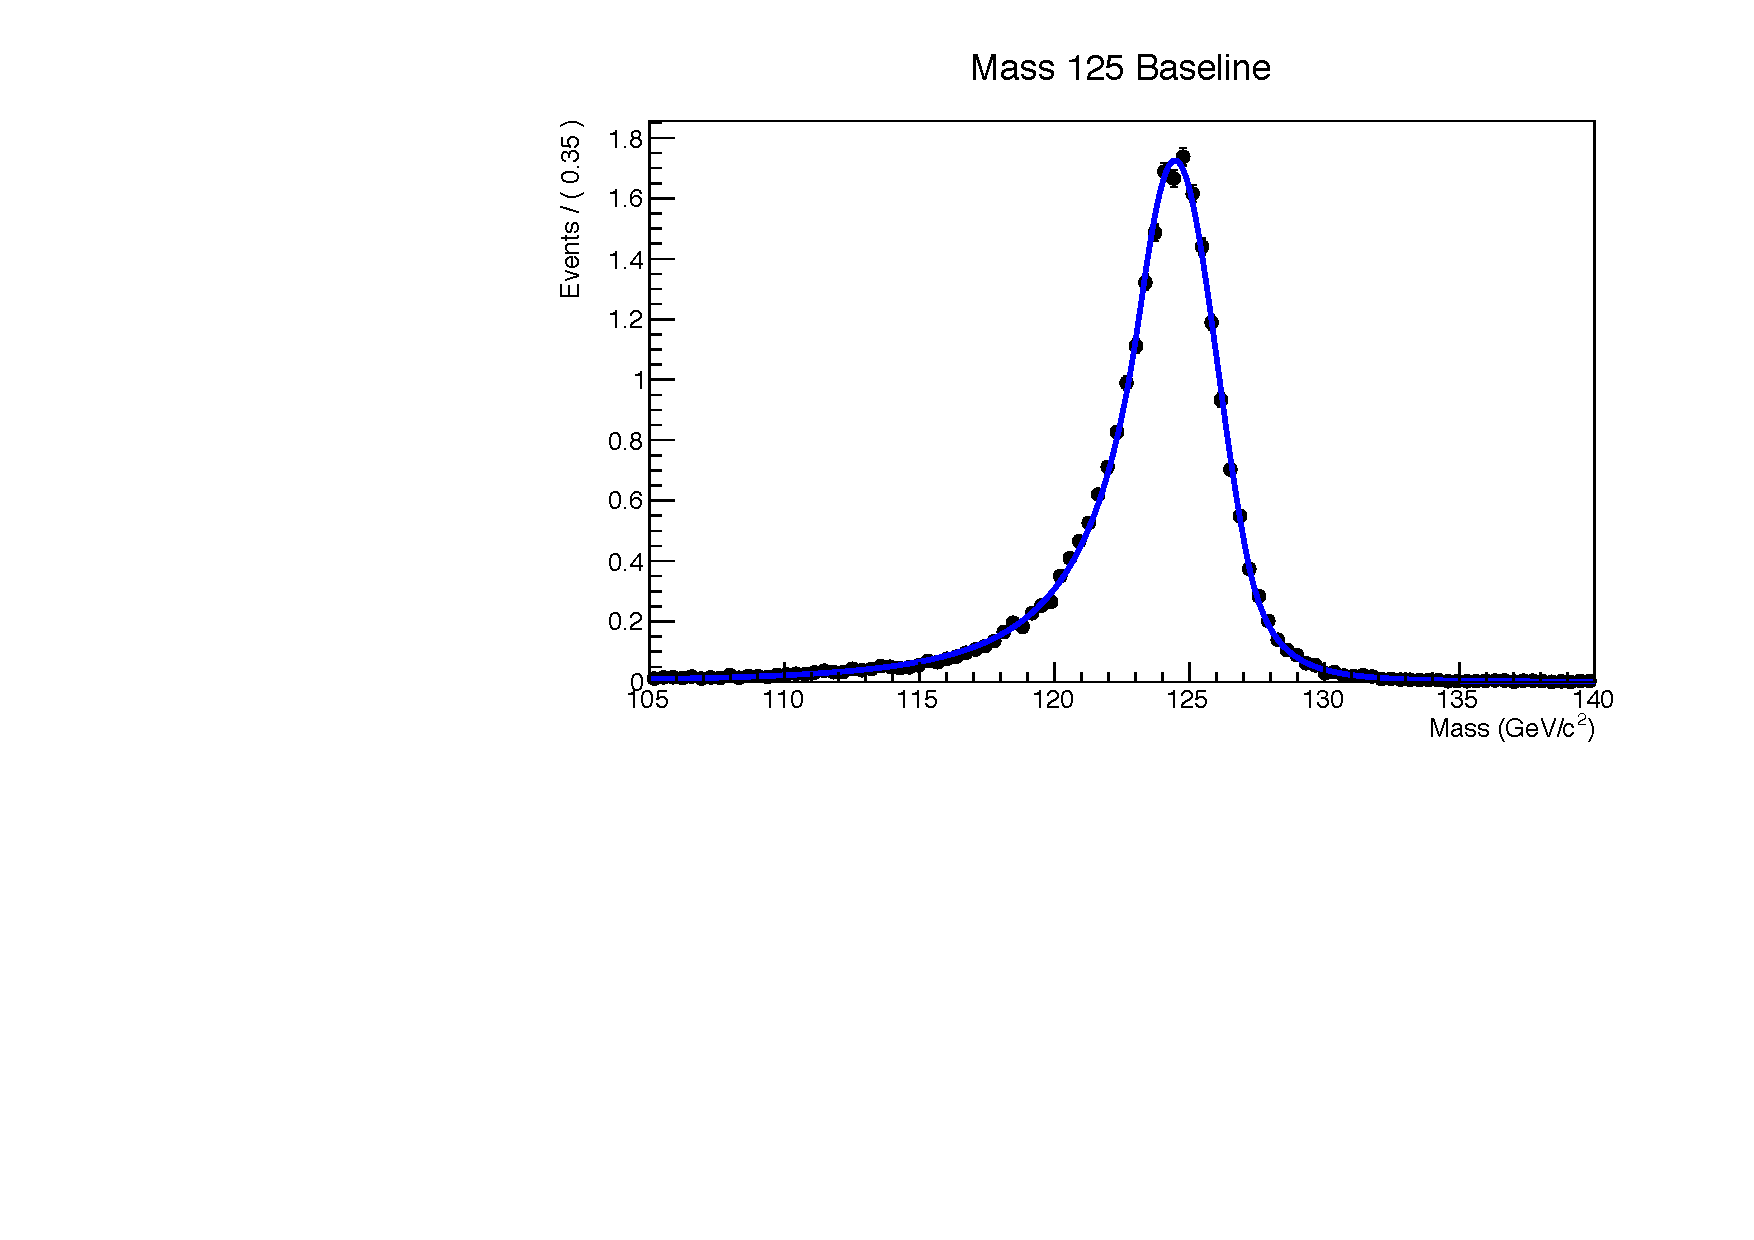
\includegraphics[width=0.3\textwidth]{../../higgsmassmeasurement/AN-19-248/Figures/SignalModelling/Signal_Parametrization/2016/ggH_2e2mu_2016_125.pdf}
%	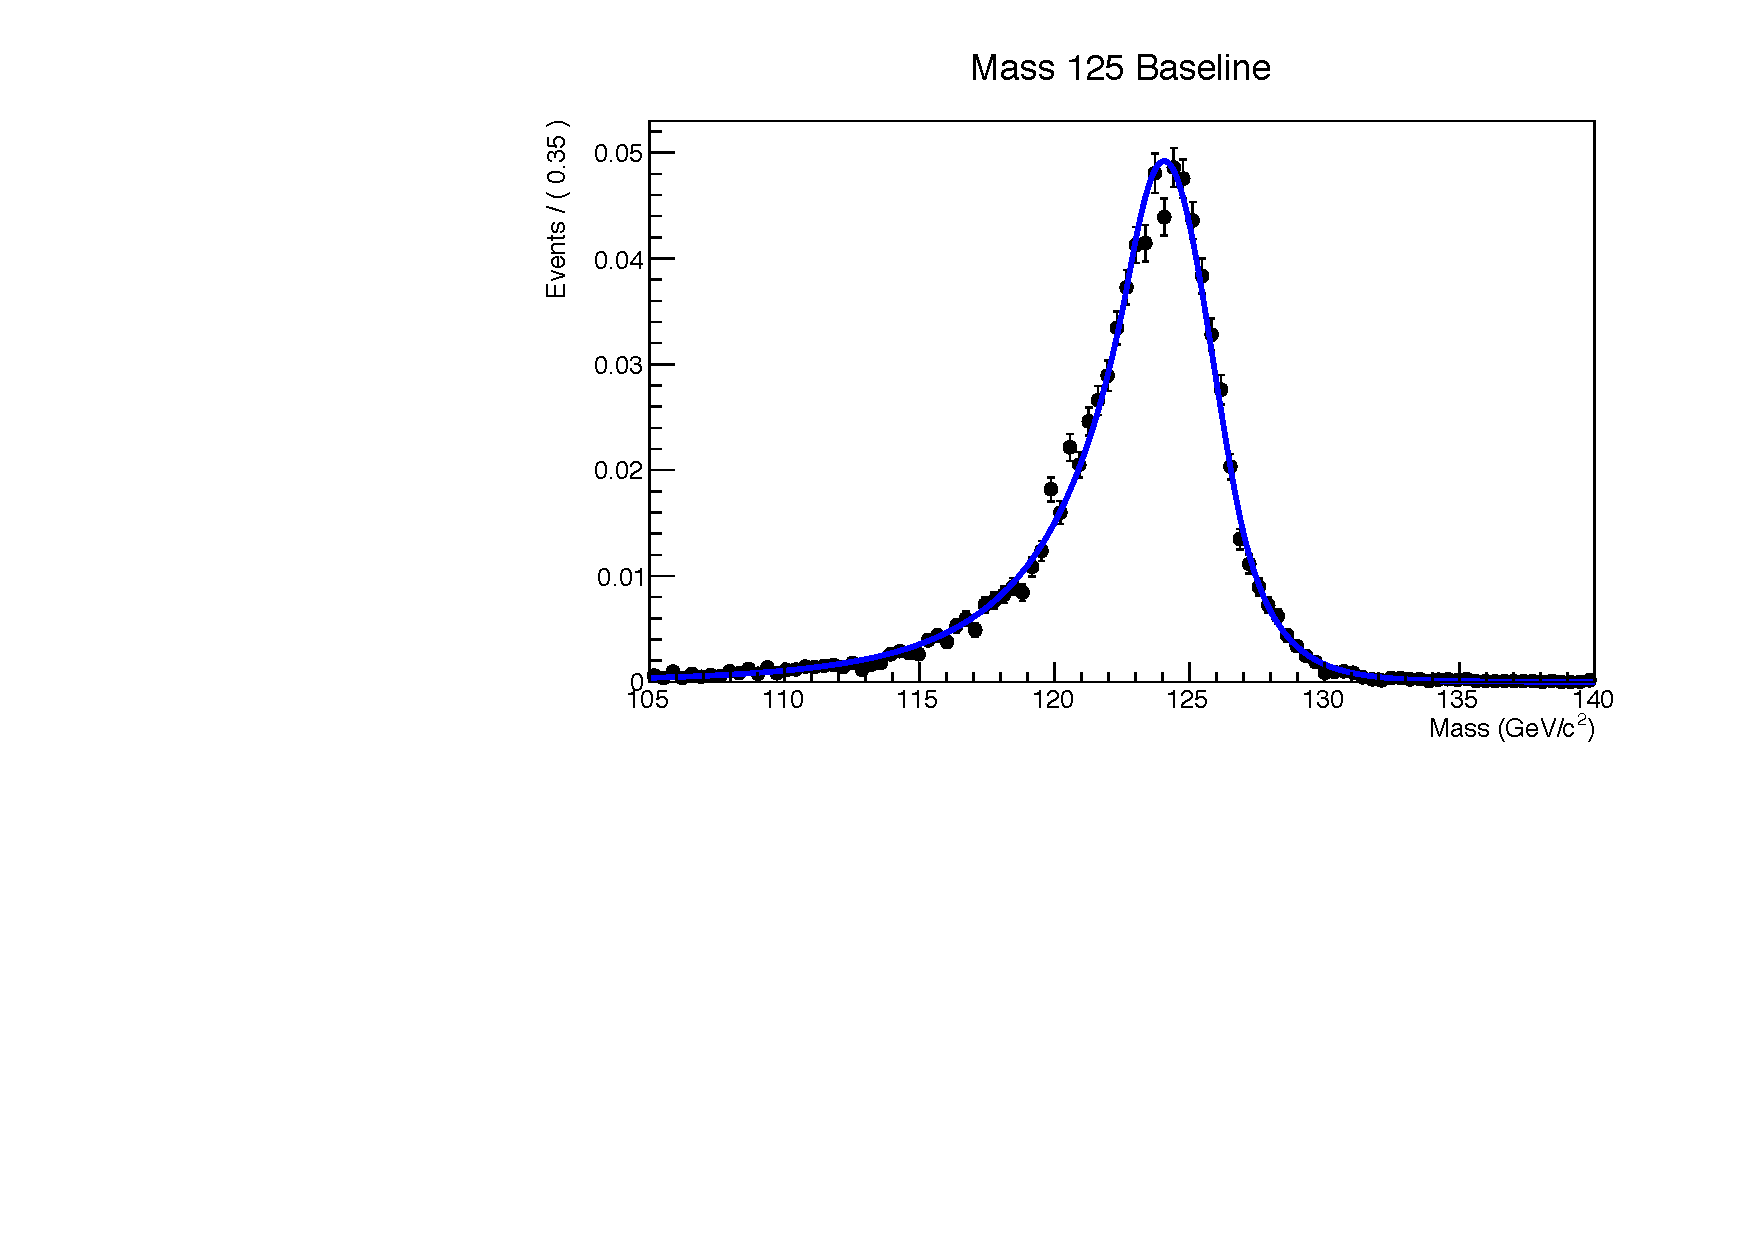
\includegraphics[width=0.3\textwidth]{../../higgsmassmeasurement/AN-19-248/Figures/SignalModelling/Signal_Parametrization/2016/VBF_4e_2016_125.pdf} 
%%		\includegraphics[width=0.3\textwidth]{../../higgsmassmeasurement/AN-19-248/Figures/SignalModelling/Signal_Parametrization/2016/2016_WH_yield.pdf}
%	\caption{125 GeV fit in 2016: 2e2$\mu$ ggH on the left, 
%	4e VBF on the right.}
%\label{signal_lineshape_2016}
%\end{center}
%\end{figure}
%\begin{figure}[!htbp]
%\begin{center}
%  		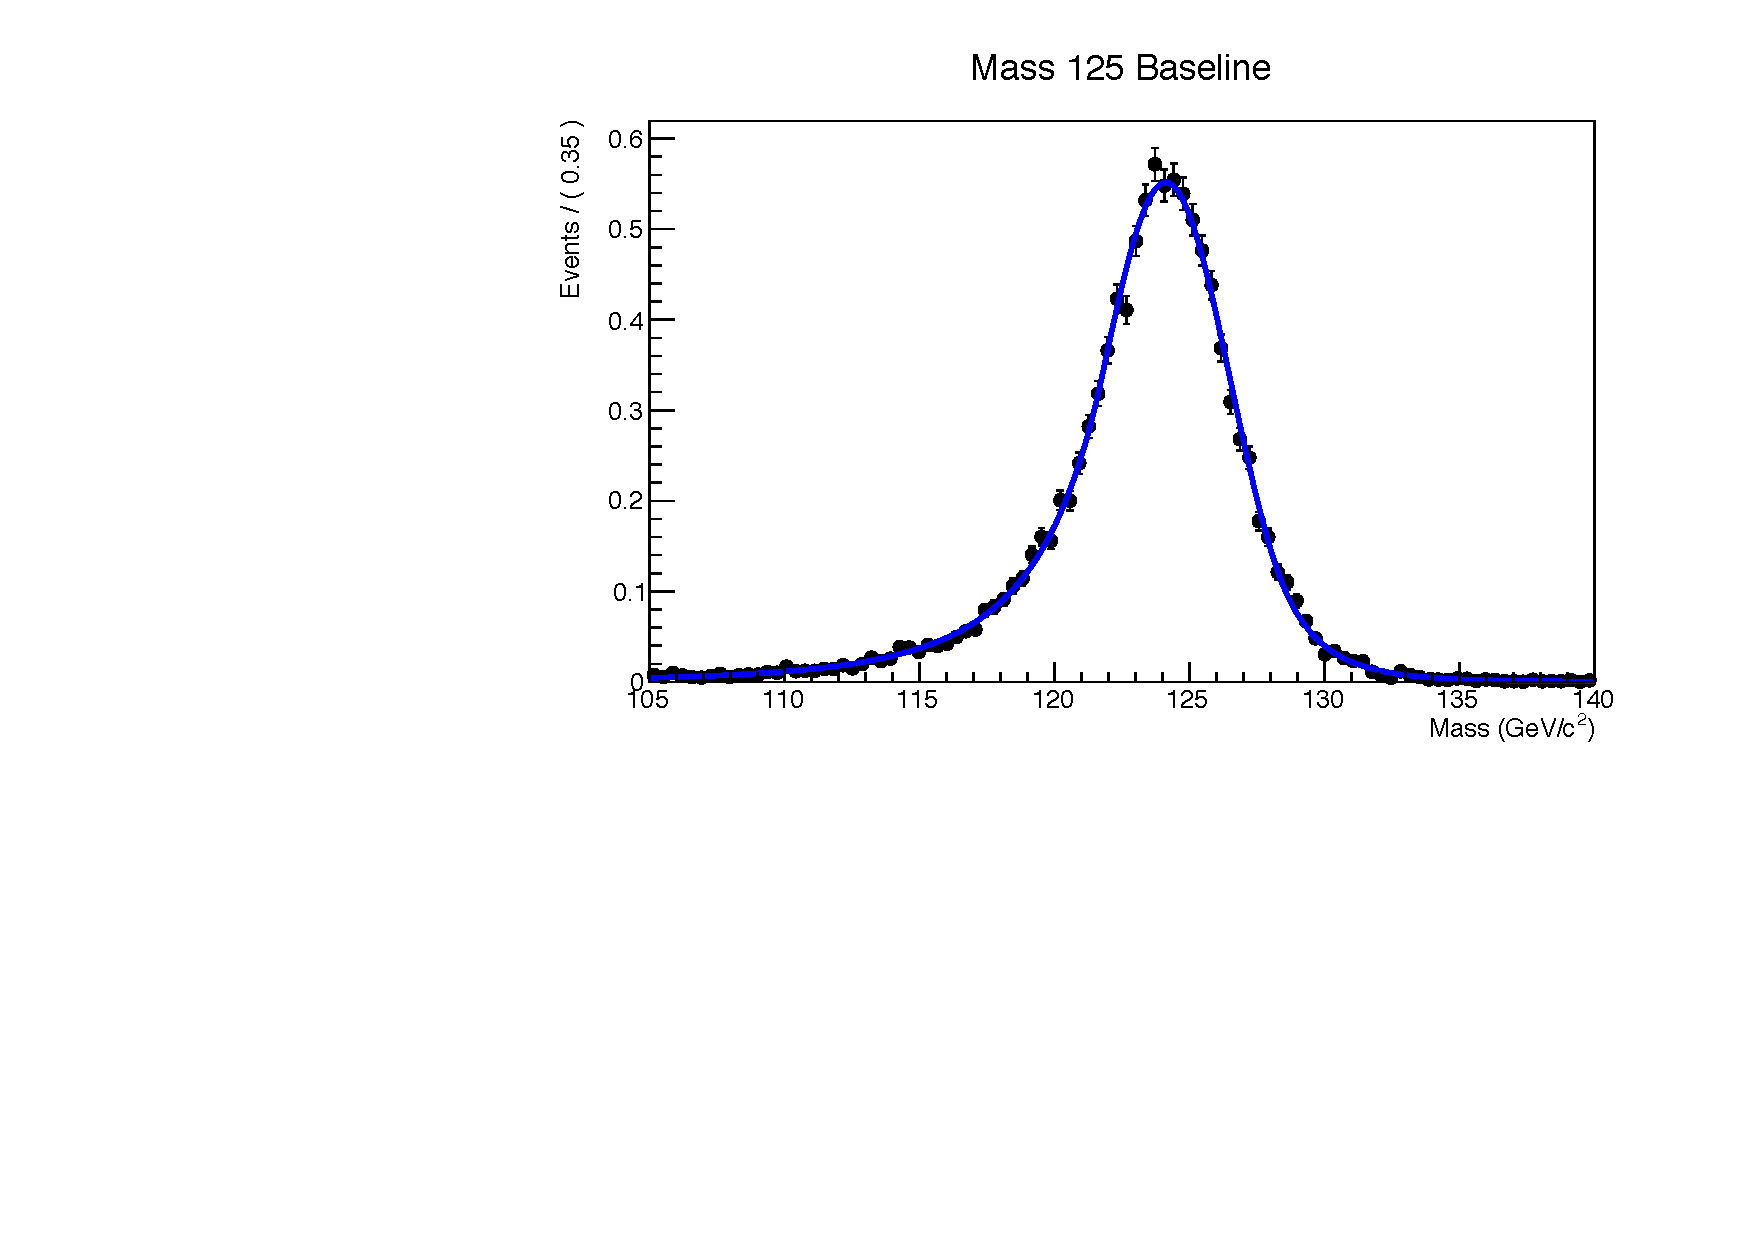
\includegraphics[width=0.3\textwidth]{../../higgsmassmeasurement/AN-19-248/Figures/SignalModelling/Signal_Parametrization/2017/ggH_4e_2017_125.pdf}
%	\includegraphics[width=0.3\textwidth]{../../higgsmassmeasurement/AN-19-248/Figures/SignalModelling/Signal_Parametrization/2017/WH_4mu_2017_125.pdf} 
%%		\includegraphics[width=0.3\textwidth]{../../higgsmassmeasurement/AN-19-248/Figures/SignalModelling/Signal_Parametrization/2017/2017_ZH_yield.pdf}
%	\caption{125 GeV fit in 2017: 4e ggH on the left, 
%	4$\mu$ WH on the right.}
%\label{signal_lineshape_2017}
%\end{center}
%\end{figure}
%\begin{figure}[!htbp]
%\begin{center}
%  		\includegraphics[width=0.3\textwidth]{../../higgsmassmeasurement/AN-19-248/Figures/SignalModelling/Signal_Parametrization/2018/ggH_4mu_2018_125.pdf}
%	\includegraphics[width=0.3\textwidth]{../../higgsmassmeasurement/AN-19-248/Figures/SignalModelling/Signal_Parametrization/2018/ttH_2e2mu_2018_125.pdf} 
%%		\includegraphics[width=0.3\textwidth]{../../higgsmassmeasurement/AN-19-248/Figures/SignalModelling/Signal_Parametrization/2017/2018_ttH_yield.pdf}
%	\caption{125 GeV fit in 2018: 4$\mu$ ggH on the left, 
%	2e2$\mu$ ttH on the right.}
%\label{signal_lineshape_2018}
%\end{center}
%\end{figure}
%
%
%\begin{figure}[!htbp]
%\begin{center}
%  		\includegraphics[width=0.3\textwidth]{../../higgsmassmeasurement/AN-19-248/Figures/SignalModelling/Signal_Parametrization/2016/ggH_2e2mu_2016_120_Sim.pdf}
%	\includegraphics[width=0.3\textwidth]{../../higgsmassmeasurement/AN-19-248/Figures/SignalModelling/Signal_Parametrization/2016/ggH_2e2mu_2016_124_Sim.pdf} 
%	\includegraphics[width=0.3\textwidth]{../../higgsmassmeasurement/AN-19-248/Figures/SignalModelling/Signal_Parametrization/2016/ggH_2e2mu_2016_125_Sim.pdf}
%	\includegraphics[width=0.3\textwidth]{../../higgsmassmeasurement/AN-19-248/Figures/SignalModelling/Signal_Parametrization/2016/ggH_2e2mu_2016_126_Sim.pdf}
%	\includegraphics[width=0.3\textwidth]{../../higgsmassmeasurement/AN-19-248/Figures/SignalModelling/Signal_Parametrization/2016/ggH_2e2mu_2016_130_Sim.pdf}
%	\caption{Simultaneous fit for ggH production mode, in 2016, for different mass points, 
%	in 2e2$\mu$ final state.}
%\label{signal_lineshape_2016_full_1}
%\end{center}
%\end{figure}
%\begin{figure}[!htbp]
%\begin{center}
%  		\includegraphics[width=0.3\textwidth]{../../higgsmassmeasurement/AN-19-248/Figures/SignalModelling/Signal_Parametrization/2016/VBF_4e_2016_120_Sim.pdf}
%	\includegraphics[width=0.3\textwidth]{../../higgsmassmeasurement/AN-19-248/Figures/SignalModelling/Signal_Parametrization/2016/VBF_4e_2016_124_Sim.pdf} 
%	\includegraphics[width=0.3\textwidth]{../../higgsmassmeasurement/AN-19-248/Figures/SignalModelling/Signal_Parametrization/2016/VBF_4e_2016_125_Sim.pdf}
%	\includegraphics[width=0.3\textwidth]{../../higgsmassmeasurement/AN-19-248/Figures/SignalModelling/Signal_Parametrization/2016/VBF_4e_2016_126_Sim.pdf}
%	\includegraphics[width=0.3\textwidth]{../../higgsmassmeasurement/AN-19-248/Figures/SignalModelling/Signal_Parametrization/2016/VBF_4e_2016_130_Sim.pdf}
%	\caption{Simultaneous fit for VBF production mode, in 2016, for different mass points, 
%	in 4e final state.}
%\label{signal_lineshape_2016_full_2}
%\end{center}
%\end{figure}
%\begin{figure}[!htbp]
%\begin{center}
%	\includegraphics[width=0.3\textwidth]{../../higgsmassmeasurement/AN-19-248/Figures/SignalModelling/Signal_Parametrization/2017/ggH_4e_2017_120_Sim.pdf}
%	\includegraphics[width=0.3\textwidth]{../../higgsmassmeasurement/AN-19-248/Figures/SignalModelling/Signal_Parametrization/2017/ggH_4e_2017_124_Sim.pdf}
%  		\includegraphics[width=0.3\textwidth]{../../higgsmassmeasurement/AN-19-248/Figures/SignalModelling/Signal_Parametrization/2017/ggH_4e_2017_125_Sim.pdf}
%	\includegraphics[width=0.3\textwidth]{../../higgsmassmeasurement/AN-19-248/Figures/SignalModelling/Signal_Parametrization/2017/ggH_4e_2017_126_Sim.pdf} 
%	\includegraphics[width=0.3\textwidth]{../../higgsmassmeasurement/AN-19-248/Figures/SignalModelling/Signal_Parametrization/2017/ggH_4e_2017_130_Sim.pdf}
%	\caption{Simultaneous fit for ggH production mode, in 2017, for different mass points, 
%	in 4e final state.}
%\label{signal_lineshape_2017_full_1}
%\end{center}
%\end{figure}
%\begin{figure}[!htbp]
%\begin{center}
%	\includegraphics[width=0.3\textwidth]{../../higgsmassmeasurement/AN-19-248/Figures/SignalModelling/Signal_Parametrization/2017/WH_4mu_2017_120_Sim.pdf}
%	\includegraphics[width=0.3\textwidth]{../../higgsmassmeasurement/AN-19-248/Figures/SignalModelling/Signal_Parametrization/2017/WH_4mu_2017_124_Sim.pdf}
%  		\includegraphics[width=0.3\textwidth]{../../higgsmassmeasurement/AN-19-248/Figures/SignalModelling/Signal_Parametrization/2017/WH_4mu_2017_125_Sim.pdf}
%	\includegraphics[width=0.3\textwidth]{../../higgsmassmeasurement/AN-19-248/Figures/SignalModelling/Signal_Parametrization/2017/WH_4mu_2017_126_Sim.pdf} 
%	\includegraphics[width=0.3\textwidth]{../../higgsmassmeasurement/AN-19-248/Figures/SignalModelling/Signal_Parametrization/2017/WH_4mu_2017_130_Sim.pdf}
%	\caption{Simultaneous fit for WH production mode, in 2017, for different mass points, 
%	in 4$\mu$ final state.}
%\label{signal_lineshape_2017_full_2}
%\end{center}
%\end{figure}
%\begin{figure}[!htbp]
%\begin{center}
%	\includegraphics[width=0.3\textwidth]{../../higgsmassmeasurement/AN-19-248/Figures/SignalModelling/Signal_Parametrization/2018/ggH_4mu_2018_120_Sim.pdf}
%	\includegraphics[width=0.3\textwidth]{../../higgsmassmeasurement/AN-19-248/Figures/SignalModelling/Signal_Parametrization/2018/ggH_4mu_2018_124_Sim.pdf}
%  		\includegraphics[width=0.3\textwidth]{../../higgsmassmeasurement/AN-19-248/Figures/SignalModelling/Signal_Parametrization/2018/ggH_4mu_2018_125_Sim.pdf}
%	\includegraphics[width=0.3\textwidth]{../../higgsmassmeasurement/AN-19-248/Figures/SignalModelling/Signal_Parametrization/2018/ggH_4mu_2018_126_Sim.pdf} 
%	\includegraphics[width=0.3\textwidth]{../../higgsmassmeasurement/AN-19-248/Figures/SignalModelling/Signal_Parametrization/2018/ggH_4mu_2018_130_Sim.pdf}
%	\caption{Simultaneous fit for ggH production mode, in 2018, for different mass points, 
%	in 4$\mu$ final state.}
%\label{signal_lineshape_2018_full_1}
%\end{center}
%\end{figure}
%\begin{figure}[!htbp]
%\begin{center}
%	\includegraphics[width=0.3\textwidth]{../../higgsmassmeasurement/AN-19-248/Figures/SignalModelling/Signal_Parametrization/2018/ttH_2e2mu_2018_120_Sim.pdf}
%	\includegraphics[width=0.3\textwidth]{../../higgsmassmeasurement/AN-19-248/Figures/SignalModelling/Signal_Parametrization/2018/ttH_2e2mu_2018_120_Sim.pdf}
%  		\includegraphics[width=0.3\textwidth]{../../higgsmassmeasurement/AN-19-248/Figures/SignalModelling/Signal_Parametrization/2018/ttH_2e2mu_2018_120_Sim.pdf}
%	\includegraphics[width=0.3\textwidth]{../../higgsmassmeasurement/AN-19-248/Figures/SignalModelling/Signal_Parametrization/2018/ttH_2e2mu_2018_120_Sim.pdf} 
%	\includegraphics[width=0.3\textwidth]{../../higgsmassmeasurement/AN-19-248/Figures/SignalModelling/Signal_Parametrization/2018/ttH_2e2mu_2018_120_Sim.pdf}
%	\caption{Simultaneous fit for ggH production mode, in 2018, for different mass points, 
%	in 2e2$\mu$ final state.}
%\label{signal_lineshape_2018_full_2}
%\end{center}
%\end{figure}

%The new four-lepton mass ($m'_{4\ell}$) and the new mass error uncertainty ($D'_{m}$), obtained after 
%the constraint of the on-shell Z boson, 
%are used to rebuilt the 2D likelihood function, $\mathcal{L}(m'_{4\ell}, D'_{m})|m_{H})$.
%The expected $\mass{H}$ measurement uncertainty, in case of no-bkg and no-syst, 
%split for different final state, is reported in
%~Table~\ref{table:2D_model_result_Z1} (or in Table~\ref{table:2D_model_result_Z1_year}
%splitted in years), compared with 2D result.
%\begin{table}[ht]	
%\begin{center}
%\begin{tabular}{|c|cccc|c|}
%\hline			
%Expected uncertainty	&	4$\mu$	&	4e	&	2e2$\mu$	&2$\mu$2e	& inclusive \\
%\hline			
%2D model with Z1 constraint	&	-	&	-	&	-	&	-	&	-	\\
%2D model	&	-	&	-	&	-	&	-	&	-	\\
%\hline
%relative improvement	&	-	&	-	&	-	&	-	&	-	\\
%\hline
%\end{tabular}
%\end{center}
%\caption{Higgs boson mass uncertainty measured with 2D model, with and without the Z1 constraint. 
%	All mass values are given in \GeV.  
%	The uncertainties are the total statistical plus systematic uncertainty, unless otherwise stated.}
%\label{table:2D_model_result_Z1}
%\end{table}
%\begin{table}[ht]	
%\begin{center}
%\begin{tabular}{|c|ccc|c|}
%\hline			
%Expected uncertainty	&	2016	&	2017	&	2018	& inclusive	\\
%\hline			
%2D model with Z1 constraint	&	-	&	-	&	-	&	-	\\
%2D model	&	-	&	-	&	-	&	-	\\
%\hline
%relative improvement	&	-	&	-	&	-	&	-	\\
%\hline
%\end{tabular}
%\end{center}
%\caption{Higgs boson mass uncertainty measured with 2D model, with and without the Z1 constraint. 
%	All mass values are given in \GeV.  
%	The uncertainties are the total statistical plus systematic uncertainty, unless otherwise stated.}
%\label{table:2D_model_result_Z1_year}
%\end{table}
%
%Next step will be to taken into account also the new muon reconstruction. 
%Final 2D model ($\mathcal{L}(m'^{~VX+BS}_{4\ell}, D'^{~VX+BS}_{m}|m_{H})$) 
%results are shown in Table~\ref{table:2D_model_result_Z1_MuonRefit}
%(or in Table~\ref{table:2D_model_result_Z1_MuonRefit_year} split in year), 
%compared with previous result.
%\begin{table}[ht]	
%\begin{center}
%\begin{tabular}{|c|cccc|c|}
%\hline			
%Expected uncertainty	&	4$\mu$	&	4e	&	2e2$\mu$	&2$\mu$2e	& inclusive	\\
%\hline			
%2D model (with Z1 and muon refit)	&	-	&	-	&	-	&	-	&	-	\\
%2D model (with Z1)	&	-	&	-	&	-	&	-	&	-	\\
%\hline
%relative improvement	&	-	&	-	&	-	&	-	&	-	\\
%\hline
%\end{tabular}
%\end{center}
%\caption{Higgs boson mass uncertainty measured with 2D model, with and without the new muon reconstruction.
%	All mass values are given in \GeV.  
%	The uncertainties are the total statistical plus systematic uncertainty, unless otherwise stated.}
%\label{table:2D_model_result_Z1_MuonRefit}
%\end{table}
%\begin{table}[ht]	
%\begin{center}
%\begin{tabular}{|c|ccc|c|}
%\hline			
%Expected uncertainty	&	2016	&	2017	&	2018	& inclusive	\\
%\hline			
%2D model (with Z1 and muon refit)	&	-	&	-	&	-	&	-	\\
%2D model (with Z1)	&	-	&	-	&	-	&	-	\\
%\hline
%relative improvement	&	-	&	-	&	-	&	-	\\
%\hline
%\end{tabular}
%\end{center}
%\caption{Higgs boson mass uncertainty measured with 2D model, with and without the new muon reconstruction.
%	All mass values are given in \GeV.  
%	The uncertainties are the total statistical plus systematic uncertainty, unless otherwise stated.}
%\label{table:2D_model_result_Z1_MuonRefit_year}
%\end{table}
